% !TeX spellcheck = pl_PL-Polish
\documentclass[12pt,a4paper]{article}

\usepackage[T1]{fontenc}
\usepackage[polish]{babel}
\usepackage[utf8]{inputenc}
\usepackage{lmodern}
\selectlanguage{polish}
\usepackage{graphicx}
\usepackage{xcolor}
\usepackage{float}
\usepackage[colorlinks=true, urlcolor=blue, linkcolor=black]{hyperref}

\def\projectName{Symulacja zarządzania projektem wytwarzania oprogramowania w systemie Jira}
\def\authorC{Wiktor Jarosz}
\def\authorB{Andrzej Machnik}
\def\authorA{Tomasz Solarz}
\newcommand\todo[1]{\textcolor{red}{#1}}

\begin{document}
\pagenumbering{gobble}
\clearpage
	\begin{figure}[h]
		\centering
		%
\includegraphics[width=0.5\linewidth]{media/polsl_logo_pion_en_rgb.png}
		
\includegraphics[width=0.5\linewidth]{media/ps-logo.png}
	\end{figure}

\hspace{3cm}
	\begin{center}Dokumentacja projektowa\end{center}
	\hspace{3cm}
	\begin{center}\large\textbf{Zarządzanie Systemami Informatycznymi}\end{center}
	\begin{center}\large\textit{\projectName}\end{center}

\hspace{7cm}
	\begin{flushright}Kierunek: Informatyka
		\end{flushright}
		\begin{flushright}Członkowie zespołu:
		\par
		\textit{\authorC}
		\par
		\textit{\authorB}
		\par
		\textit{\authorA}
	\end{flushright}
\vfill
	\begin{center}Gliwice, 2025/2026\end{center}

\newpage
\pagenumbering{arabic}
\tableofcontents





\newpage
\section{Wprowadzenie}
\subsection{Role w projekcie}
	W ramach projektu przyjęto następujący podział ról w zespole projektowym (Scrum Team):
	\begin{itemize}
		\item \textbf{Tomasz Solarz} -- Scrum Master / Developer
		\item \textbf{Andrzej Machnik} -- Developer
		\item \textbf{Wiktor Jarosz} -- Product Owner / Developer
	\end{itemize}
	Ze względu na niewielki, trzyosobowy zespół, każdy z członków aktywnie uczestniczył w wytwarzaniu oprogramowania na stanowisku Developera, jednocześnie pełniąc kluczowe role wspierające proces zarządzania (Scrum Master, Product Owner).

\subsection{Cel projektu}
	Celem projektu była symulacja małego projektu z wytwarzania oprogramowania przy użyciu platformy Jira w ramach zwinnej metodyki Scrum. Naszym zadaniem było przeprowadzenie procesu twórczego na przestrzeni kilku sprintów oraz praktyczne wykorzystanie i zaprezentowanie różnorodnych funkcjonalności oferowanych przez system Jira. Skupiliśmy się na takich elementach jak planowanie sprintów, zarządzanie backlogiem, automatyzacje przepływu pracy, zarządzanie wydaniami oraz generowanie raportów postępów pracy zespołu.





\newpage
\section{Założenia projektowe}
\subsection{Założenia techniczne i nietechniczne}
	\begin{itemize}
		\item Organizacja pracy w metodyce zwinnej (Agile/Scrum).
		\item Zdefiniowanie przejrzystego przepływu pracy opartego o kolumny: To Do, In Progress, In Review oraz Done.
		\item Wykorzystanie elastycznego systemu zadań składającego się z Epiców, Historyjek (Story) oraz Podzadań (Subtasks).
		\item Wdrożenie automatyzacji w celu przyspieszenia powtarzalnych procesów, takich jak automatyczne zamykanie nadrzędnych zadań po ukończeniu przypisanych im podzadań.
		\item Mierzenie efektywności zespołu (Capacity/Velocity) za pomocą punktów Story Points.
		\item Usprawnienie komunikacji poprzez przeprowadzanie regularnych spotkań typu Daily Stand-up z wykorzystaniem tablicy oraz osi czasu w Jira.
	\end{itemize}

\subsection{Stos technologiczny}
	Zasadniczym narzędziem do realizacji procesu zarządzania projektem i dokumentowania przebiegu prac był system \textbf{Jira Software} w wersji cloud. Wykorzystano też funkcje raportowania natywnie wbudowane w narzędzie.

\subsection{Oczekiwane rezultaty projektu}
	Oczekiwanym efektem końcowym jest zorganizowany, kompletny projekt w narzędziu Jira odzwierciedlający cykl życia oprogramowania poprzez trzy iteracje (Sprint 0, Sprint 1, Sprint 2). Rezultaty obejmują w szczególności zaplanowane wydania (Releases), poprawnie działające automatyzacje procesów oraz realne, adekwatne dane na wykresach raportowych (Burnup, Sprint Burndown, Velocity chart), potwierdzające sprawną realizację założonego harmonogramu.





\newpage
\section{Realizacja projektu}
	W ramach realizacji projektu pomyślnie przeszliśmy przez pełny cykl konfiguracji i prowadzenia projektu w systemie Jira. Poniżej przedstawiono poszczególne kroki i etapy wraz z ilustrującymi je zrzutami ekranu z wykonanej symulacji.

	\subsection{Konfiguracja początkowa i zespół}
	Na samym początku projektu skonfigurowano pustą tablicę Scrumową z podziałem na kolumny ułatwiające orientację w procesie: \textit{To Do}, \textit{In Progress}, \textit{In Review} oraz \textit{Done} (Rysunek \ref{fig:1}). Następnie wysłano zaproszenia do pozostałych członków zespołu, tak by wszyscy mogli dołączyć do jednej, spójnej przestrzeni roboczej projektu (Rysunek \ref{fig:2}).

	\begin{figure}[H]
		\centering
		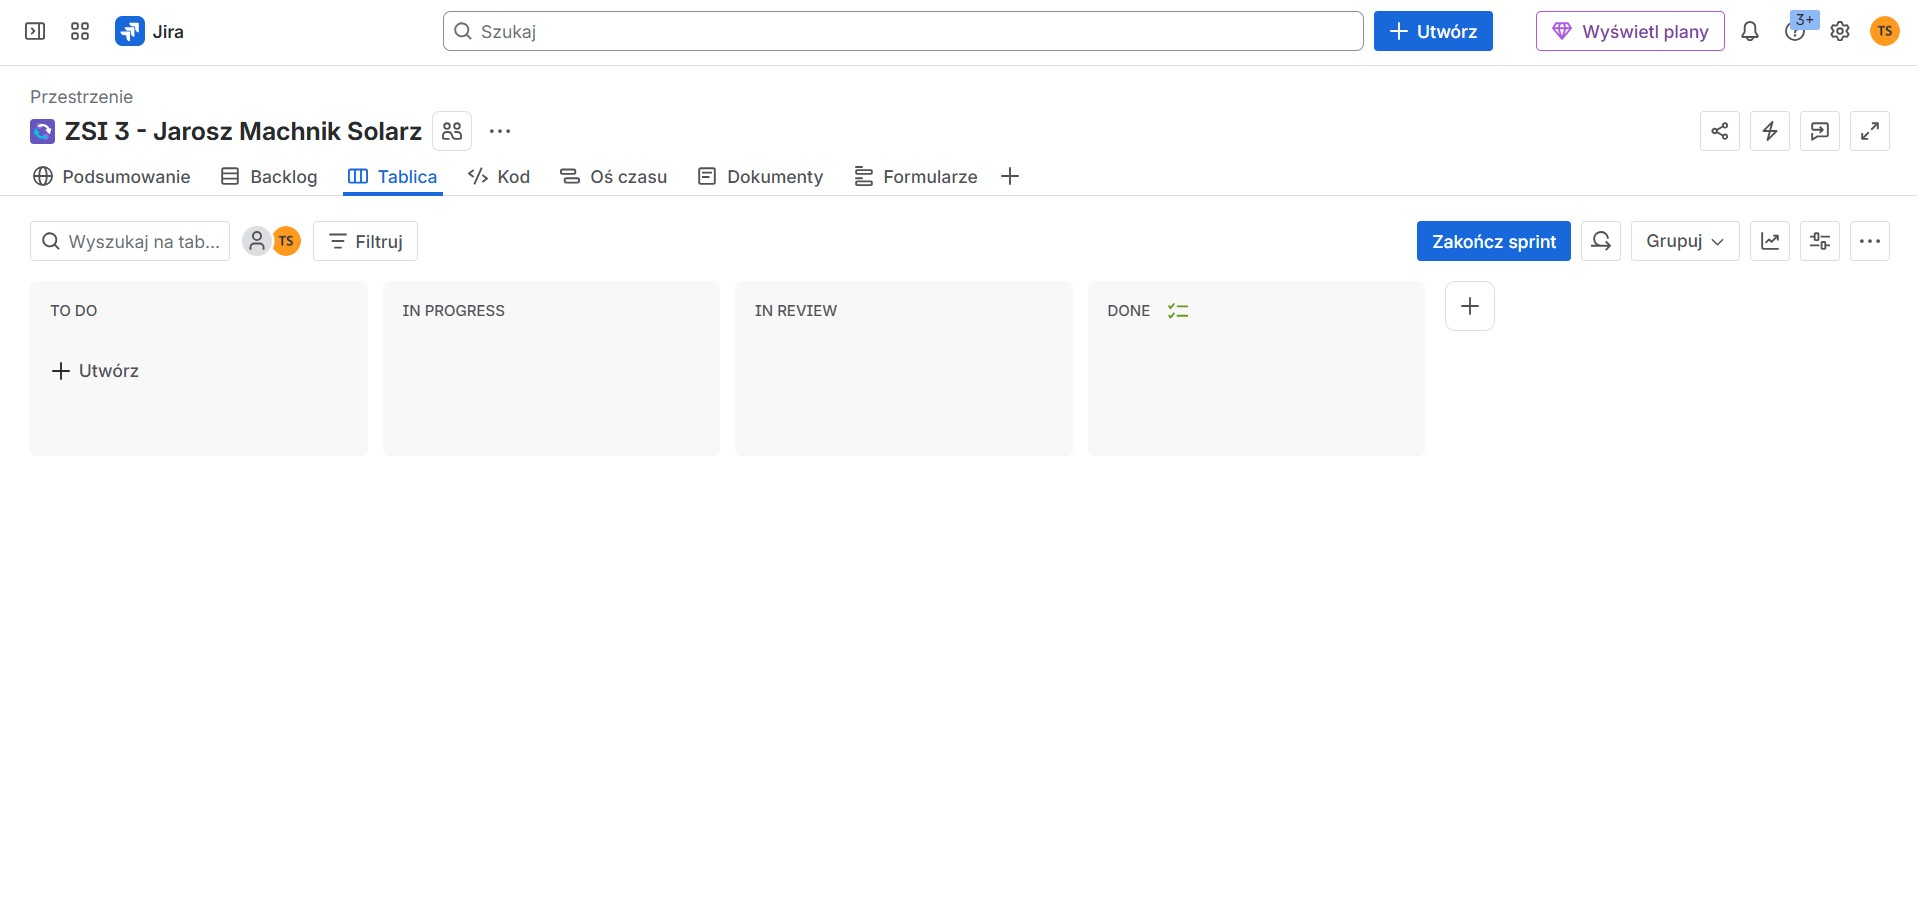
\includegraphics[width=0.8\linewidth]{../screeny/1.jpg}
		\caption{Skonfigurowana pusta tablica projektowa z podziałem na kolumny}
		\label{fig:1}
	\end{figure}

	\begin{figure}[H]
		\centering
		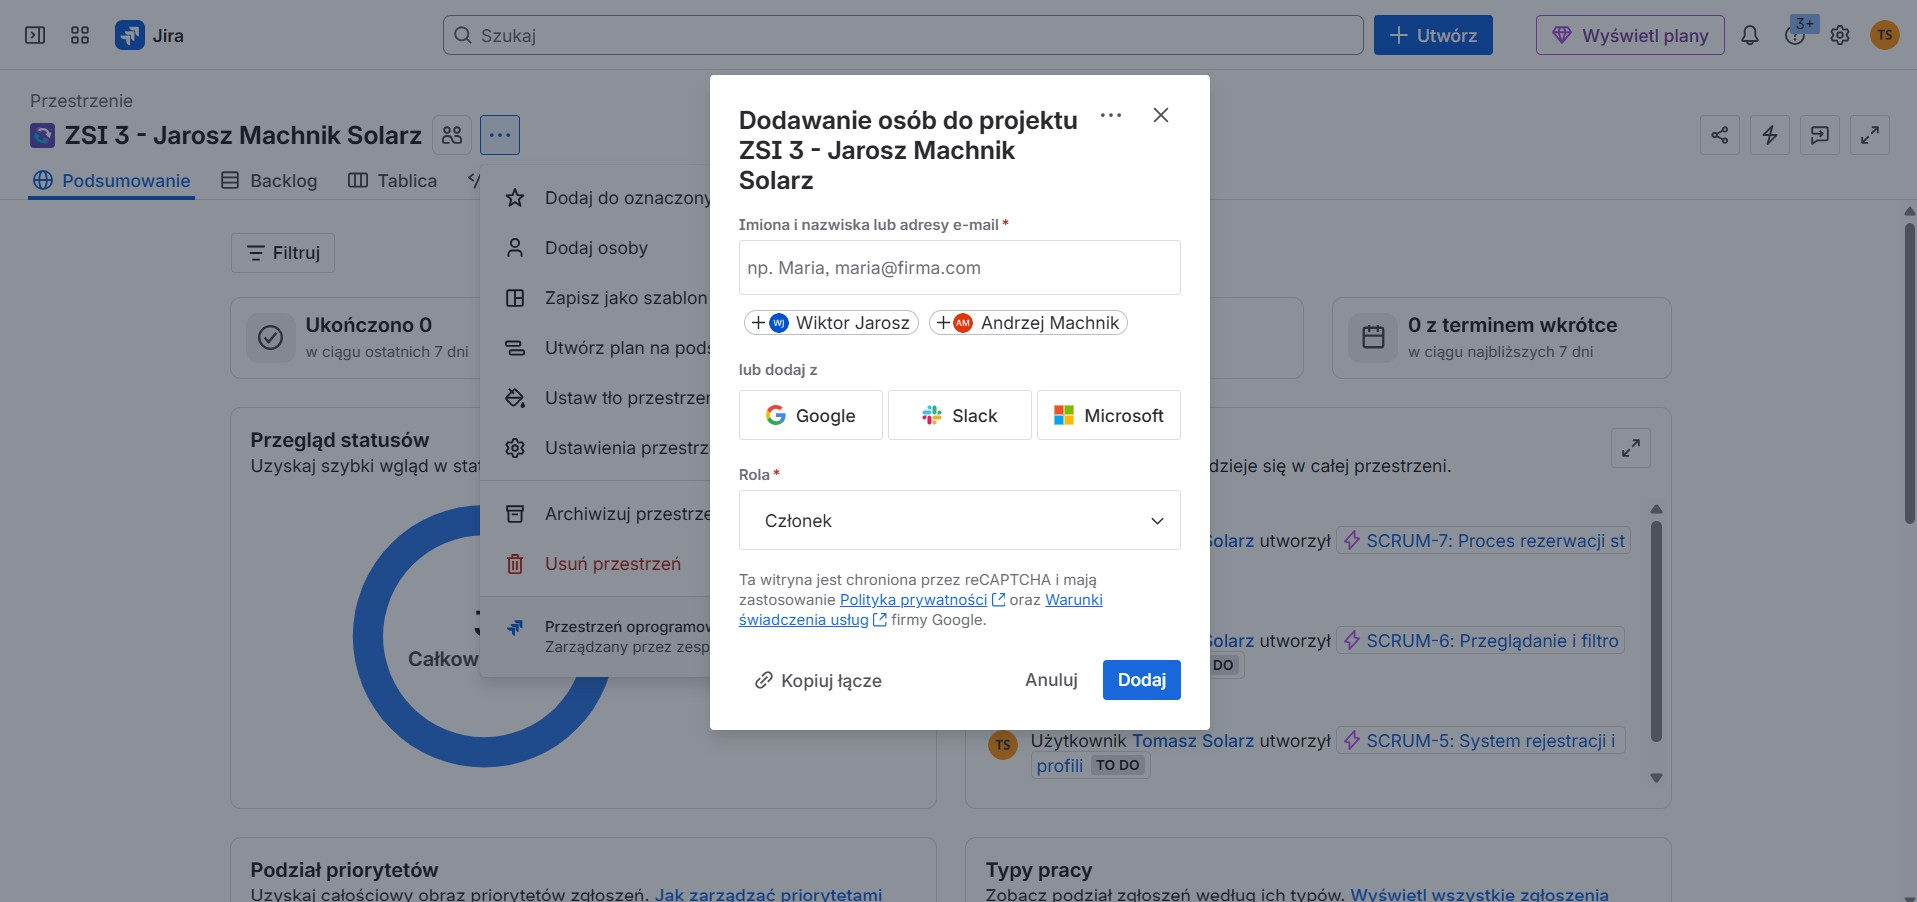
\includegraphics[width=0.8\linewidth]{../screeny/2.jpg}
		\caption{Wysyłanie zaproszeń umożliwiających dołączenie do projektu reszcie zespołu}
		\label{fig:2}
	\end{figure}

	\subsection{Struktura zadań i planowanie wydań}
	Każda historyjka (Story) definiowana w projekcie posiadała szczegółowy opis, stosowne załączniki (na przykład makiety widoków ekranu), podzadania rozpisane na różne etapy realizacji oraz jasno zdefiniowany czas startu i termin wykonania (Rysunek \ref{fig:4}). Zaplanowano również kilka odrębnych wydań (Releases), dla których ściśle określono daty, szerszy opis oraz zakres historyjek i zadań wchodzących w skład poszczególnej wersji (Rysunek \ref{fig:5}).

	\begin{figure}[H]
		\centering
		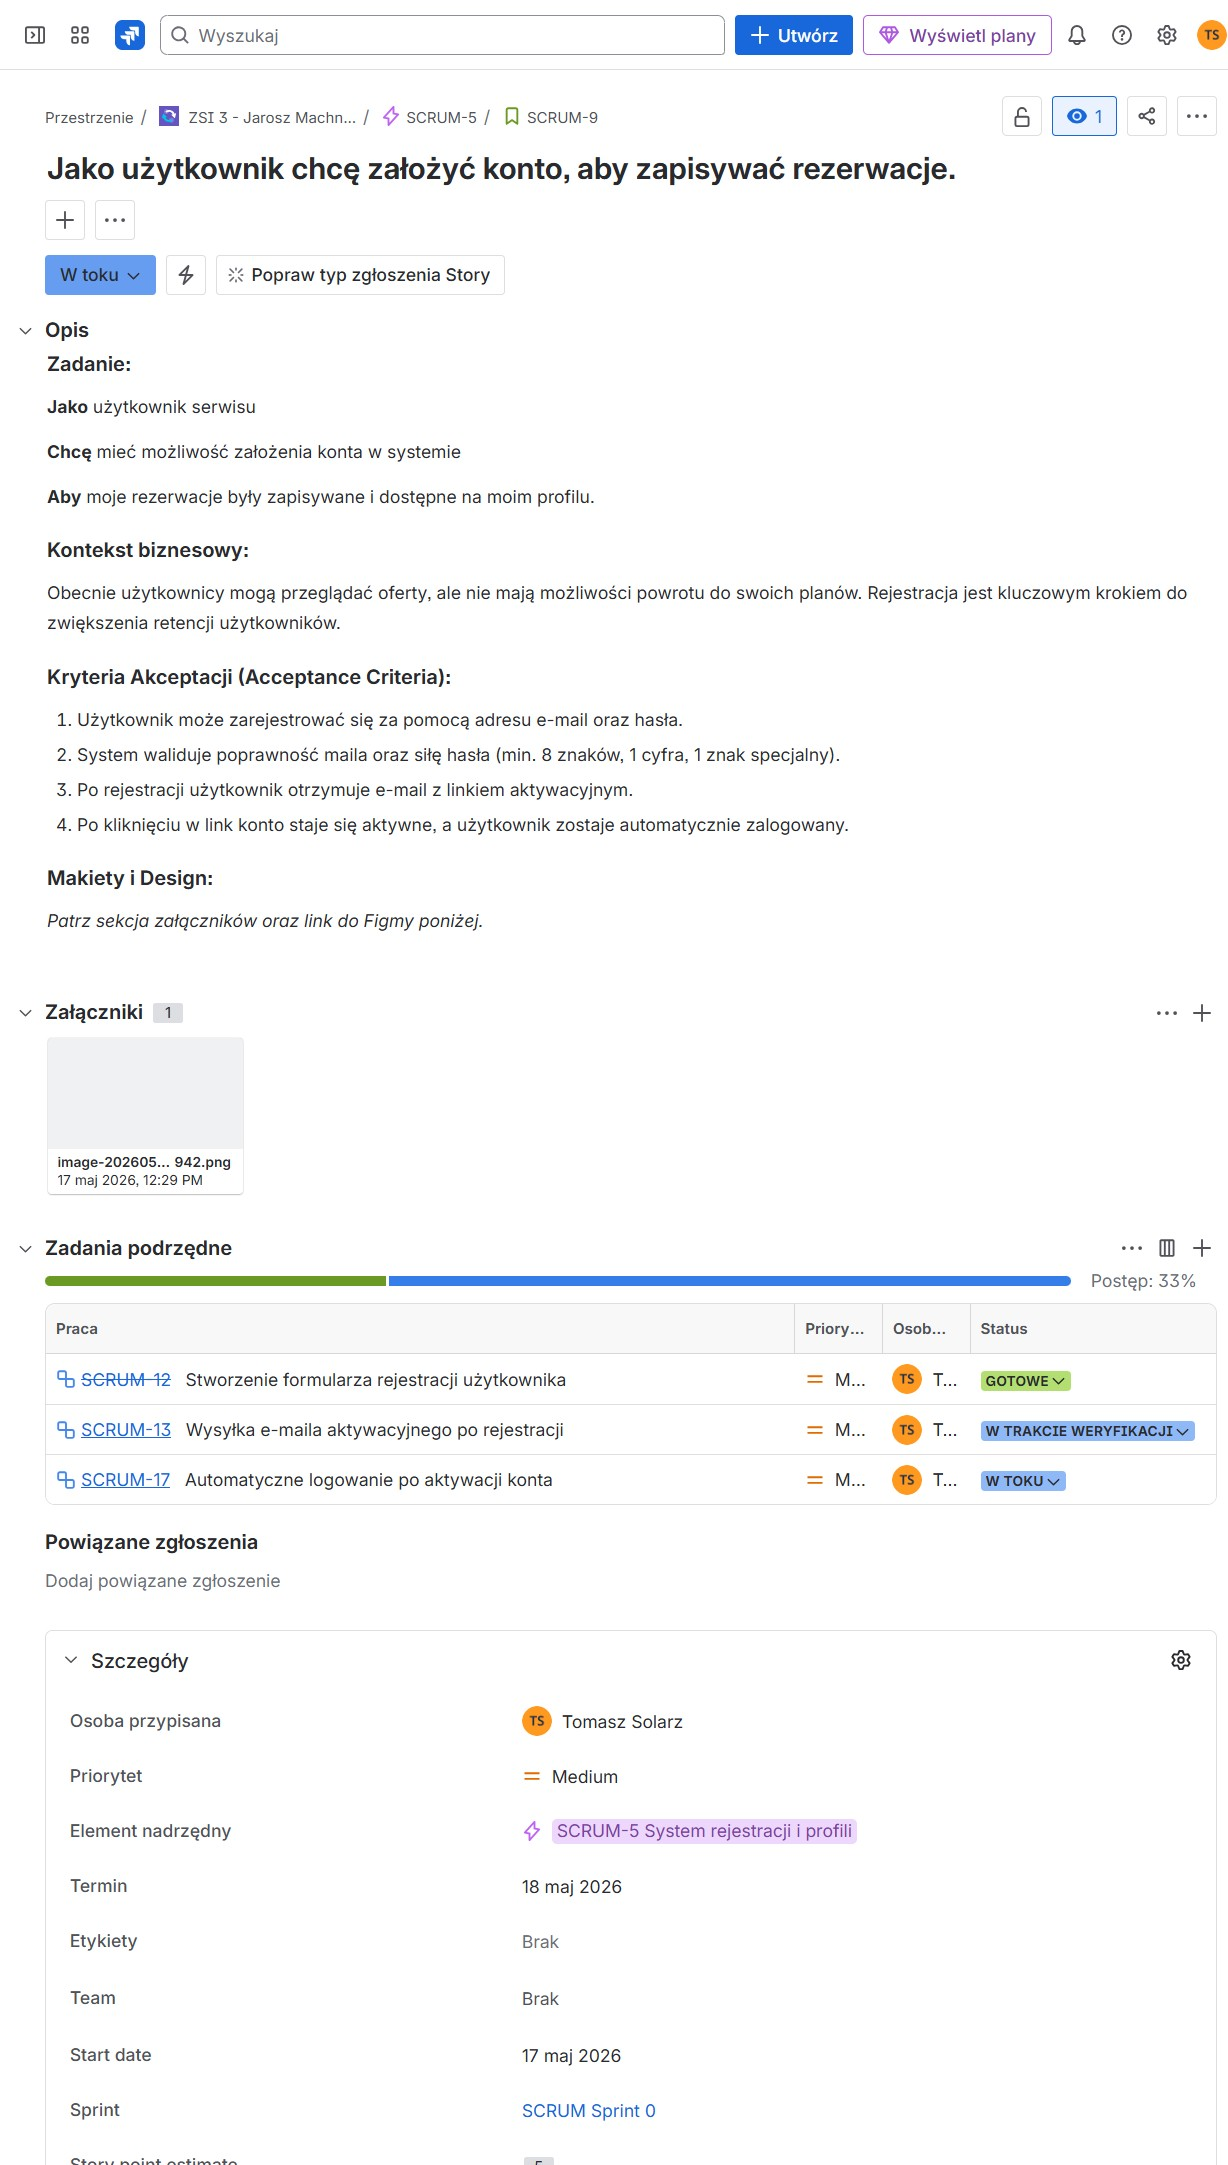
\includegraphics[width=0.8\linewidth]{../screeny/4.jpg}
		\caption{Widok szczegółowy przykładowej historyjki (Story) zawierającej podzadania oraz załączniki}
		\label{fig:4}
	\end{figure}

	\begin{figure}[H]
		\centering
		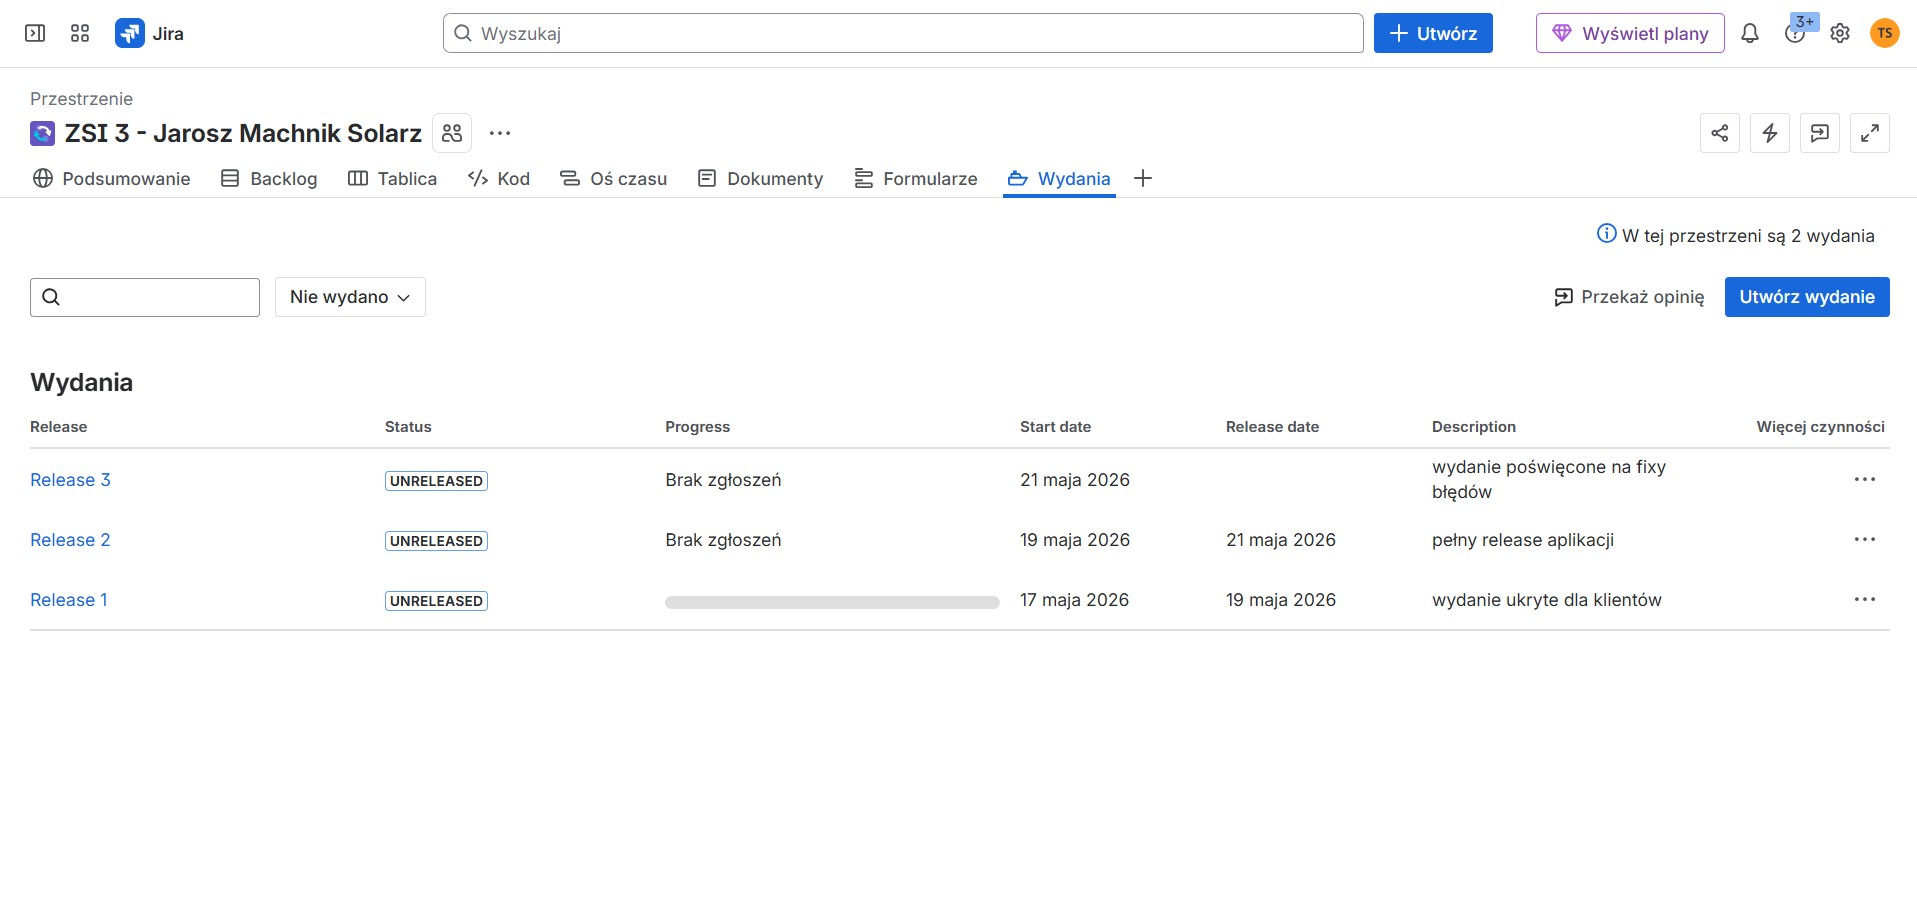
\includegraphics[width=0.8\linewidth]{../screeny/5.jpg}
		\caption{Zakładka wydań z rozplanowaniem planowanych wersji projektu}
		\label{fig:5}
	\end{figure}

	\subsection{Backlog i planowanie Sprintów}
	Naszą pracę w znacznej mierze opieraliśmy o Backlog produktu. Zawarte w nim zadania były estymowane i wyceniane za pomocą miary Story Points (SP), a po wspólnej ocenie przydzielane do poszczególnych sprintów. Na Rysunku \ref{fig:6} widoczny jest przykładowy widok zadań, które zespół wziął do sprintu o łącznej zsumowanej wycenie na 13 SP. Z kolei zakładka z osią czasu (Timeline) pozwalała nam na intuicyjną wizualizację, które zadania ostatecznie znalazły się w danym sprincie wraz z oznaczeniem ich bieżącego statusu (Rysunek \ref{fig:7}).

	\begin{figure}[H]
		\centering
		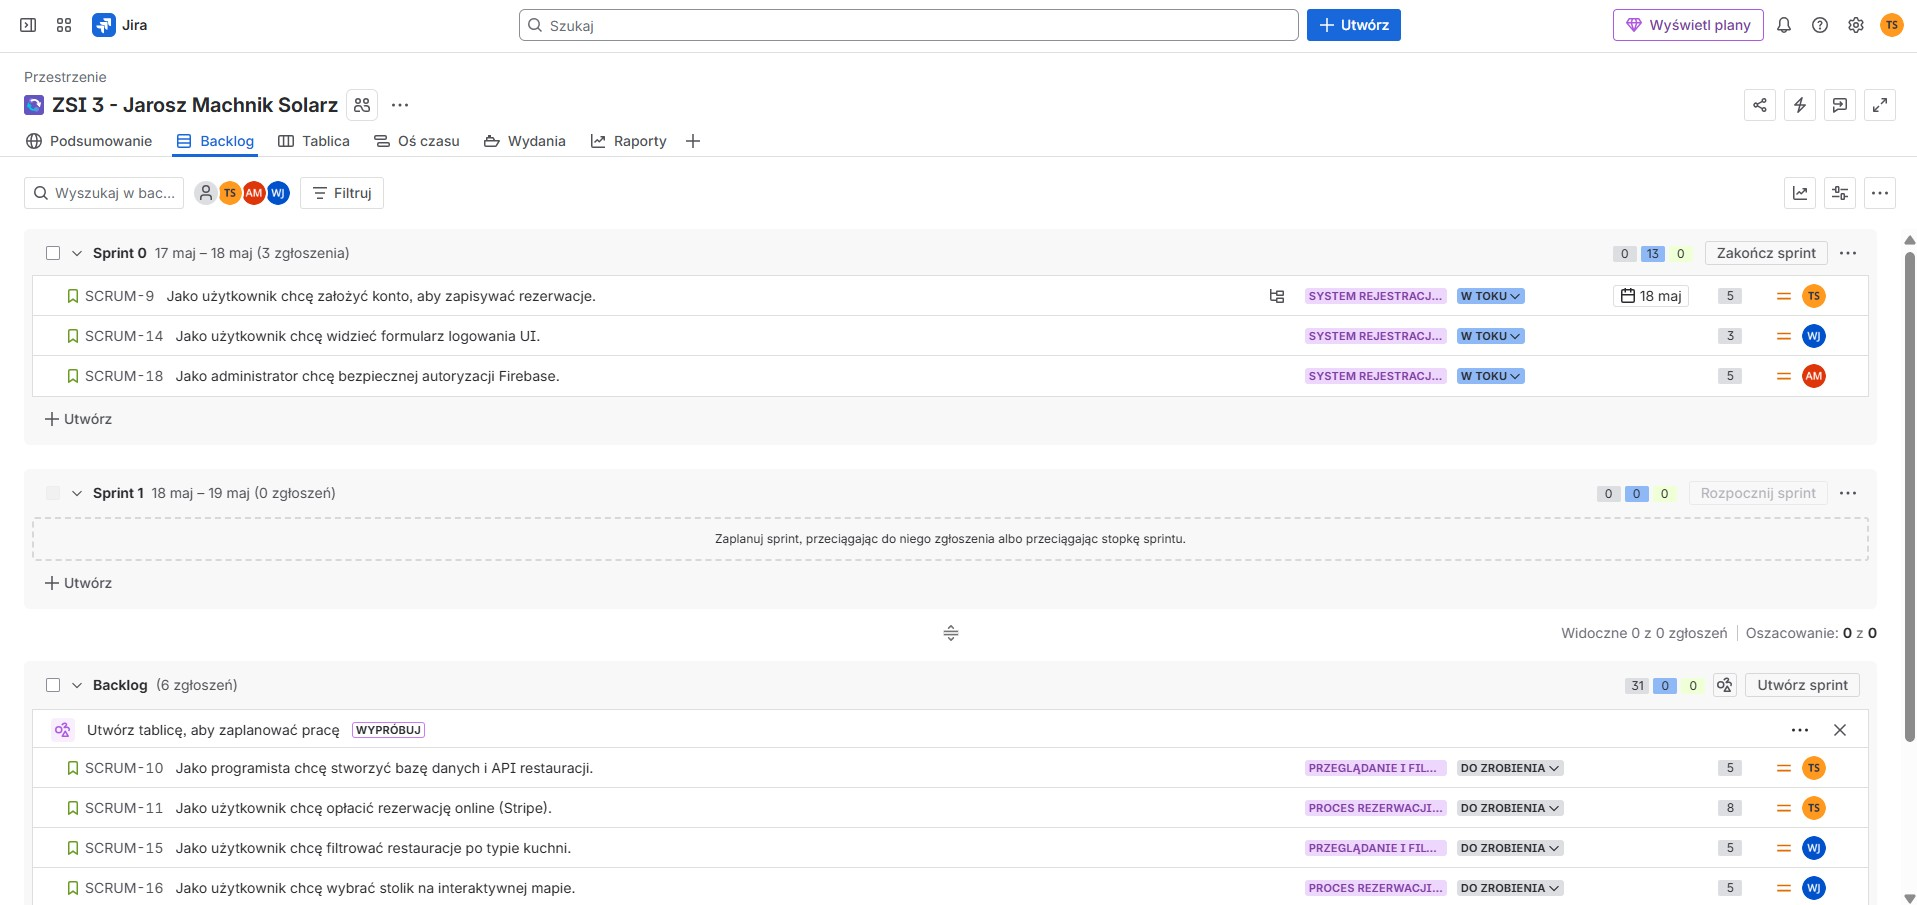
\includegraphics[width=0.8\linewidth]{../screeny/6.jpg}
		\caption{Widok Backlogu i zadań zaplanowanych do aktualnego sprintu na sumę 13 SP}
		\label{fig:6}
	\end{figure}

	\begin{figure}[H]
		\centering
		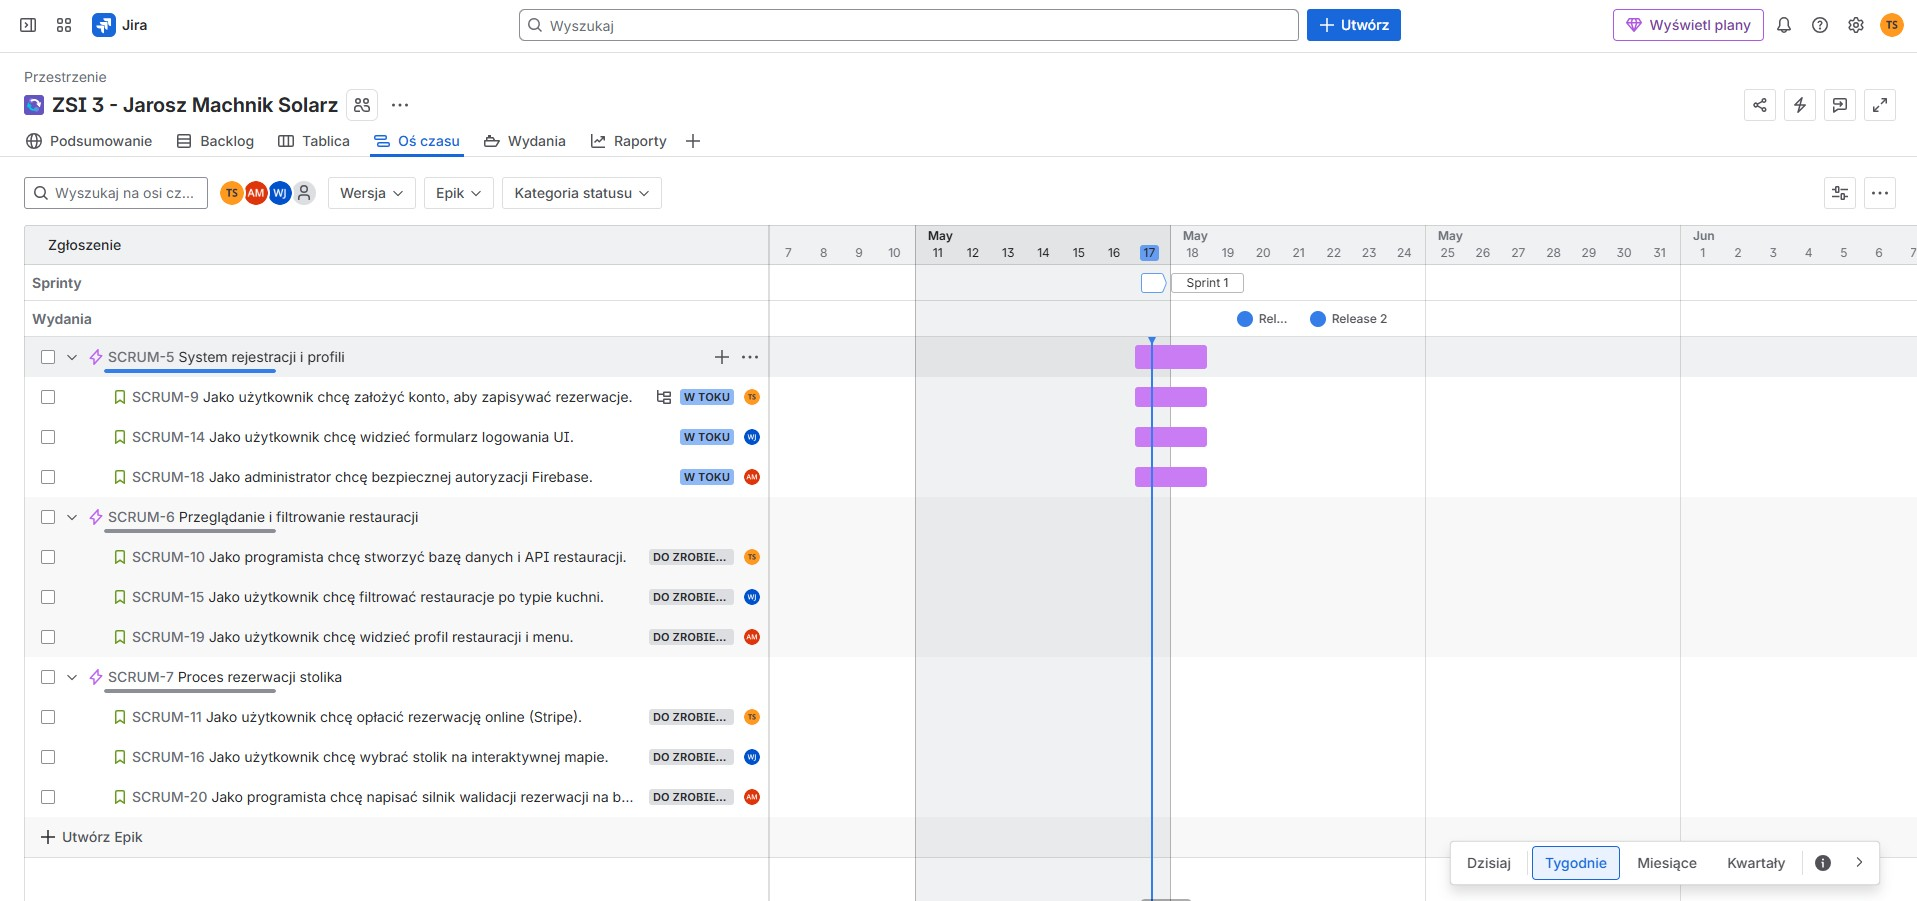
\includegraphics[width=0.8\linewidth]{../screeny/7.jpg}
		\caption{Zakładka Timeline z widokiem zadań i historyjek przyjętych do bieżącego sprintu}
		\label{fig:7}
	\end{figure}

	\subsection{Automatyzacje}
	Aby zminimalizować czynności manualne i usprawnić pracę zespołu, wprowadziliśmy systemową automatyzację, która samoczynnie zamyka danego Epica tuż po ukończeniu wszystkich przynależących podzadań. Zbudowano regułę w oparciu o silnik Automation for Jira: wyzwalaczem (Trigger) była zmiana statusu podzadania, a jako warunek (Condition) ustawiono weryfikację, czy wszystkie pozostałe podzadania powiązane z nadrzędnym Epicem znajdują się już w statusie \textit{Done}. Akcją (Action) była natychmiastowa tranzycja zadania nadrzędnego. Na Rysunku \ref{fig:3} widnieje podgląd interfejsu konfiguracyjnego podczas tworzenia tej reguły. Poprawność jej działania potwierdza widoczny wpis w logu audytu (Rysunek \ref{fig:9}), na którym zarejestrowano automatyczne przeniesienie historyjki do statusu \textit{Gotowe}. Ponadto, system generował powiadomienia e-mail potwierdzające zamknięcie historyjki dla członków zespołu (Rysunek \ref{fig:10}).

	\begin{figure}[H]
		\centering
		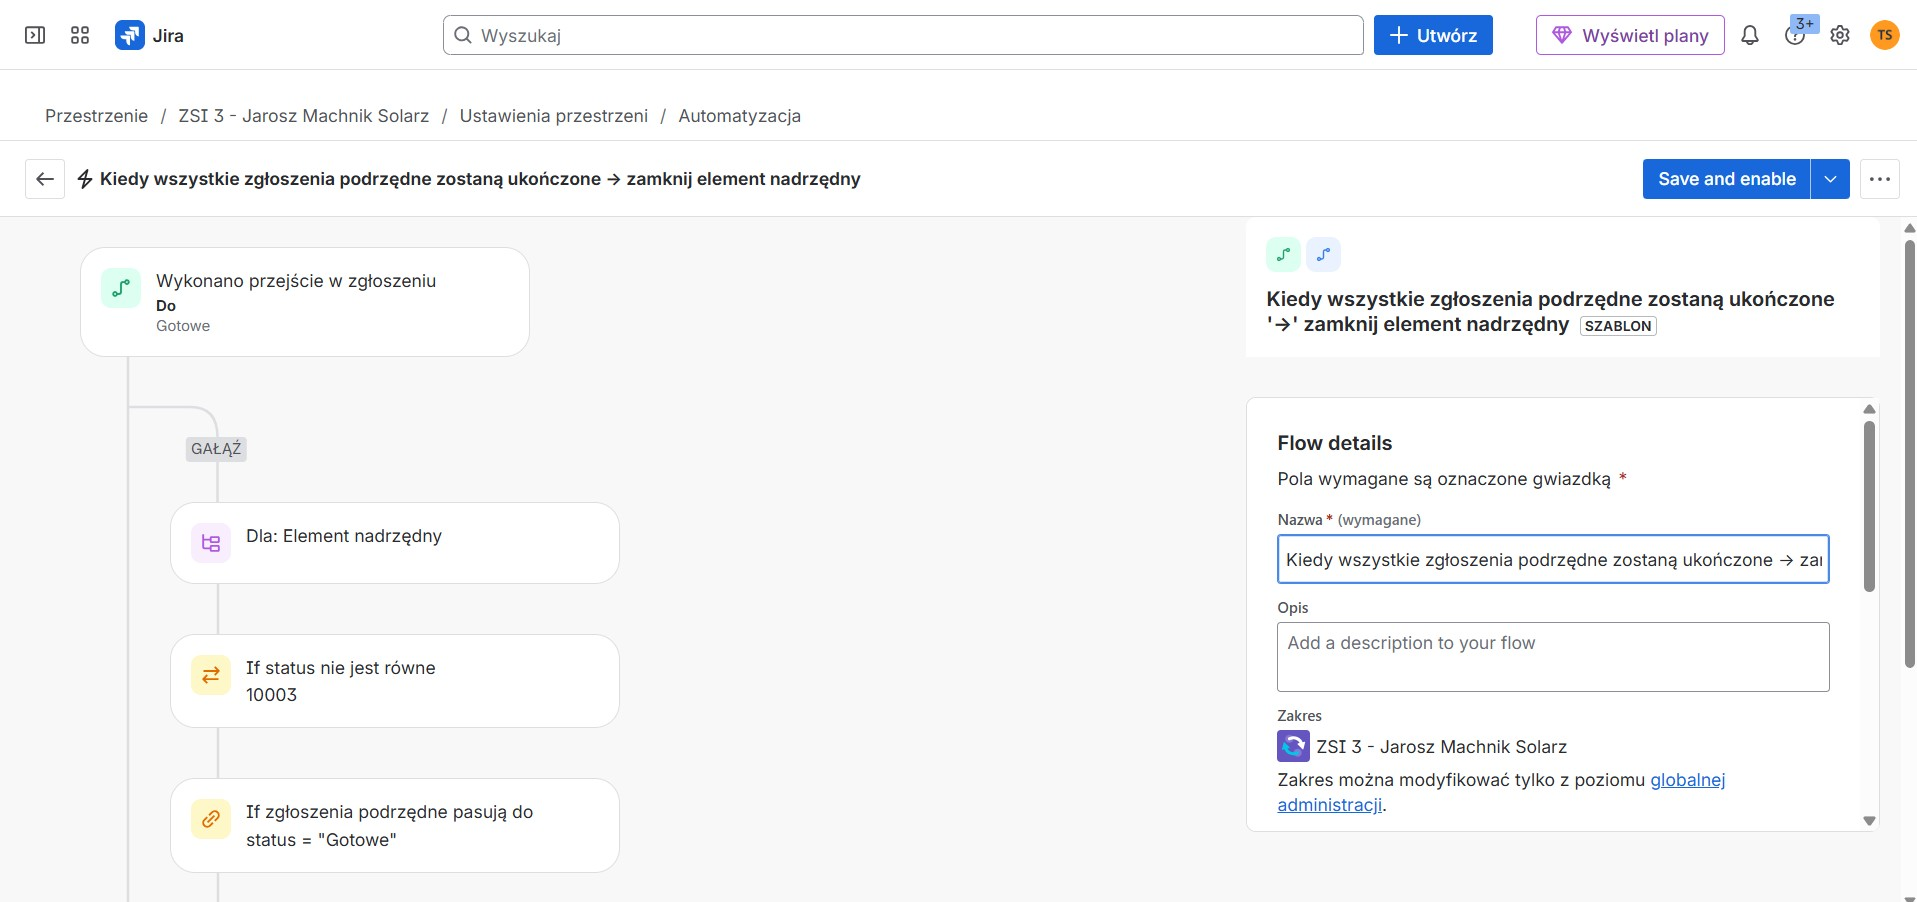
\includegraphics[width=0.8\linewidth]{../screeny/3.jpg}
		\caption{Proces tworzenia reguły automatyzacji domykającej zrealizowane Epici}
		\label{fig:3}
	\end{figure}

	\begin{figure}[H]
		\centering
		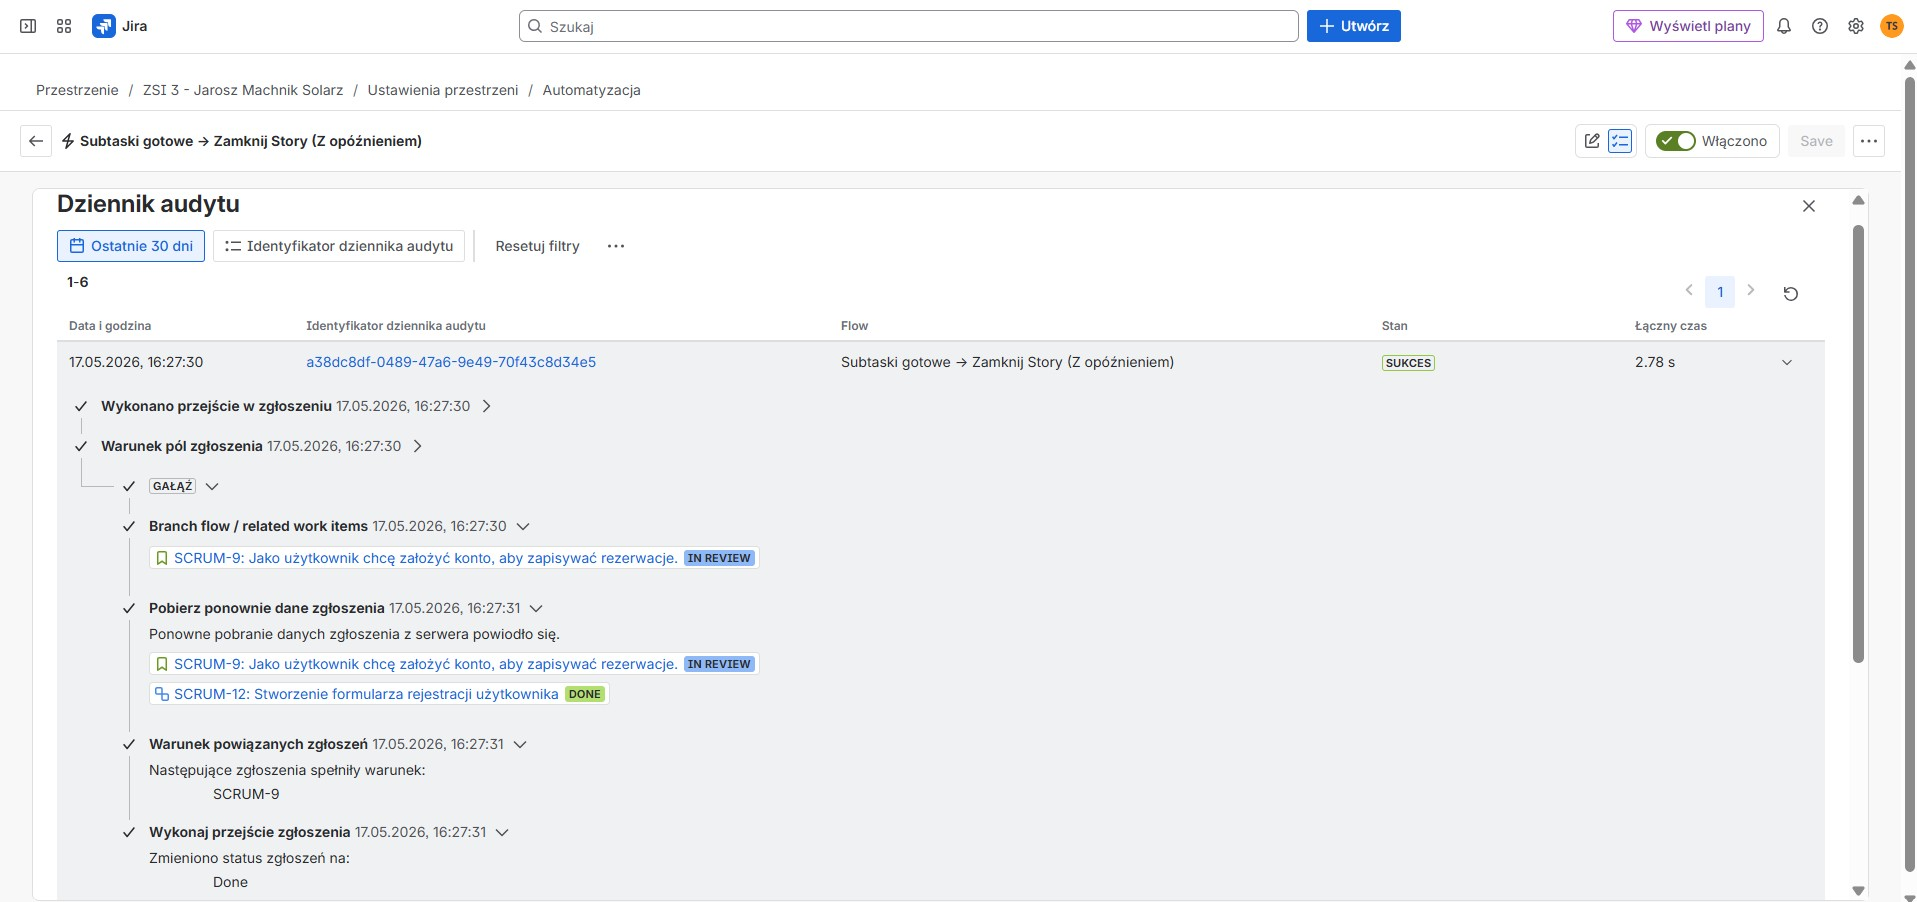
\includegraphics[width=0.8\linewidth]{../screeny/9.jpg}
		\caption{Log audytu weryfikujący poprawność działania skonfigurowanej automatyzacji}
		\label{fig:9}
	\end{figure}

	\begin{figure}[H]
		\centering
		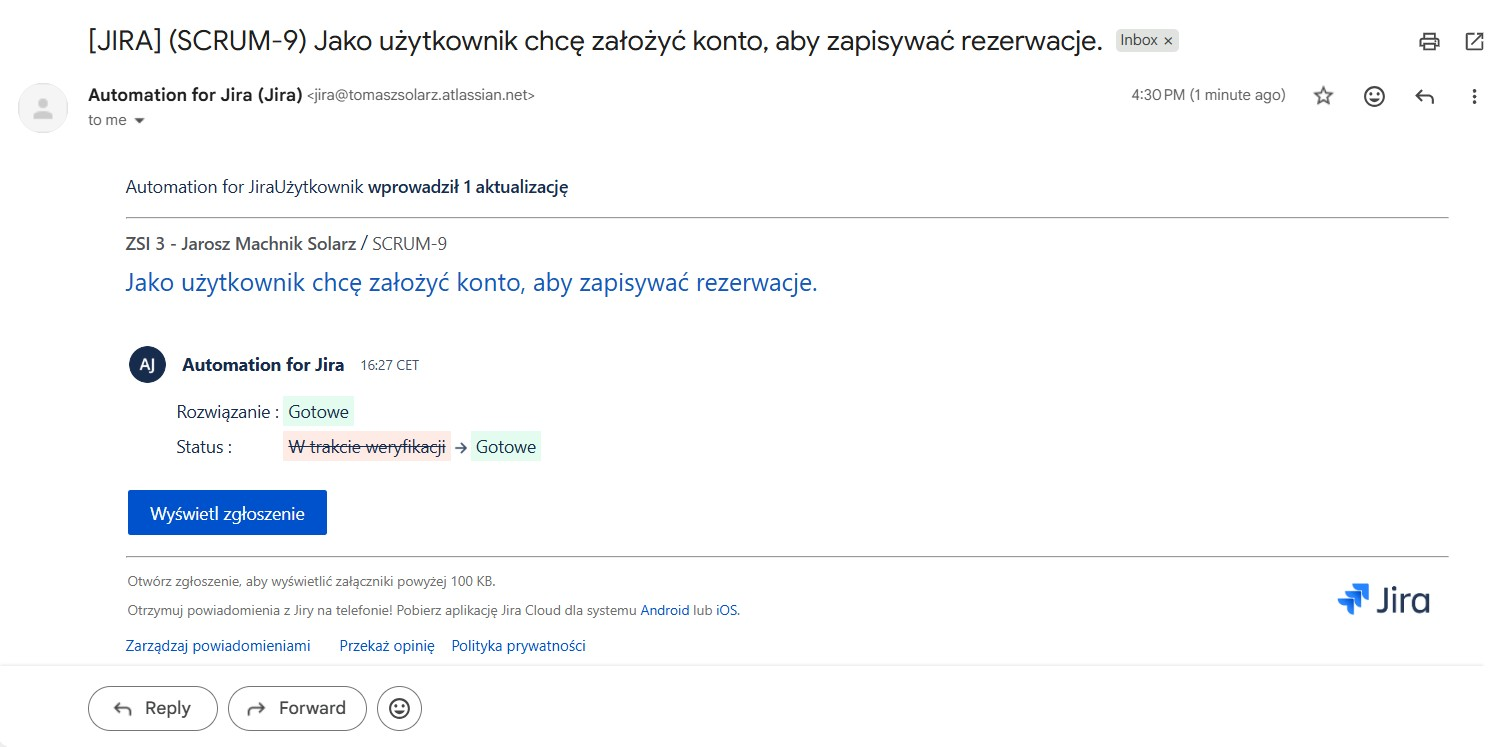
\includegraphics[width=0.8\linewidth]{../screeny/10.jpg}
		\caption{Powiadomienie mailowe wygenerowane z systemu Jira w wyniku działania automatyzacji}
		\label{fig:10}
	\end{figure}

	\subsection{Przebieg Sprintów i spotkania codzienne (Stand-up)}
	W trakcie pracy nad sprintami regularnie odbywały się zsynchronizowane spotkania Daily Stand-up. Widok z przykładowego spotkania, na którym raportowano przebieg zadań poszczególnych deweloperów (na Rysunku \ref{fig:8} widać perspektywę zadań Andrzeja, przy czym Wiktor i Tomasz zdążyli już zabrać głos), prezentował aktualny status i pozwalał koordynować dalsze prace. Z kolei Rysunek \ref{fig:11} przedstawia statystyki zaraz po całkowitym ukończeniu pierwszego sprintu weryfikacyjnego (tzw. Sprint 0). W toku projektu zdarzały się naturalnie sytuacje, w których nie wszystkie zadania udawało się dostarczyć na czas jak zadanie SCRUM-19 zaplanowane na Sprint 1 zostało przeniesione do Sprintu 2 z powodu opóźnień (Rysunek \ref{fig:12}).

	\begin{figure}[H]
		\centering
		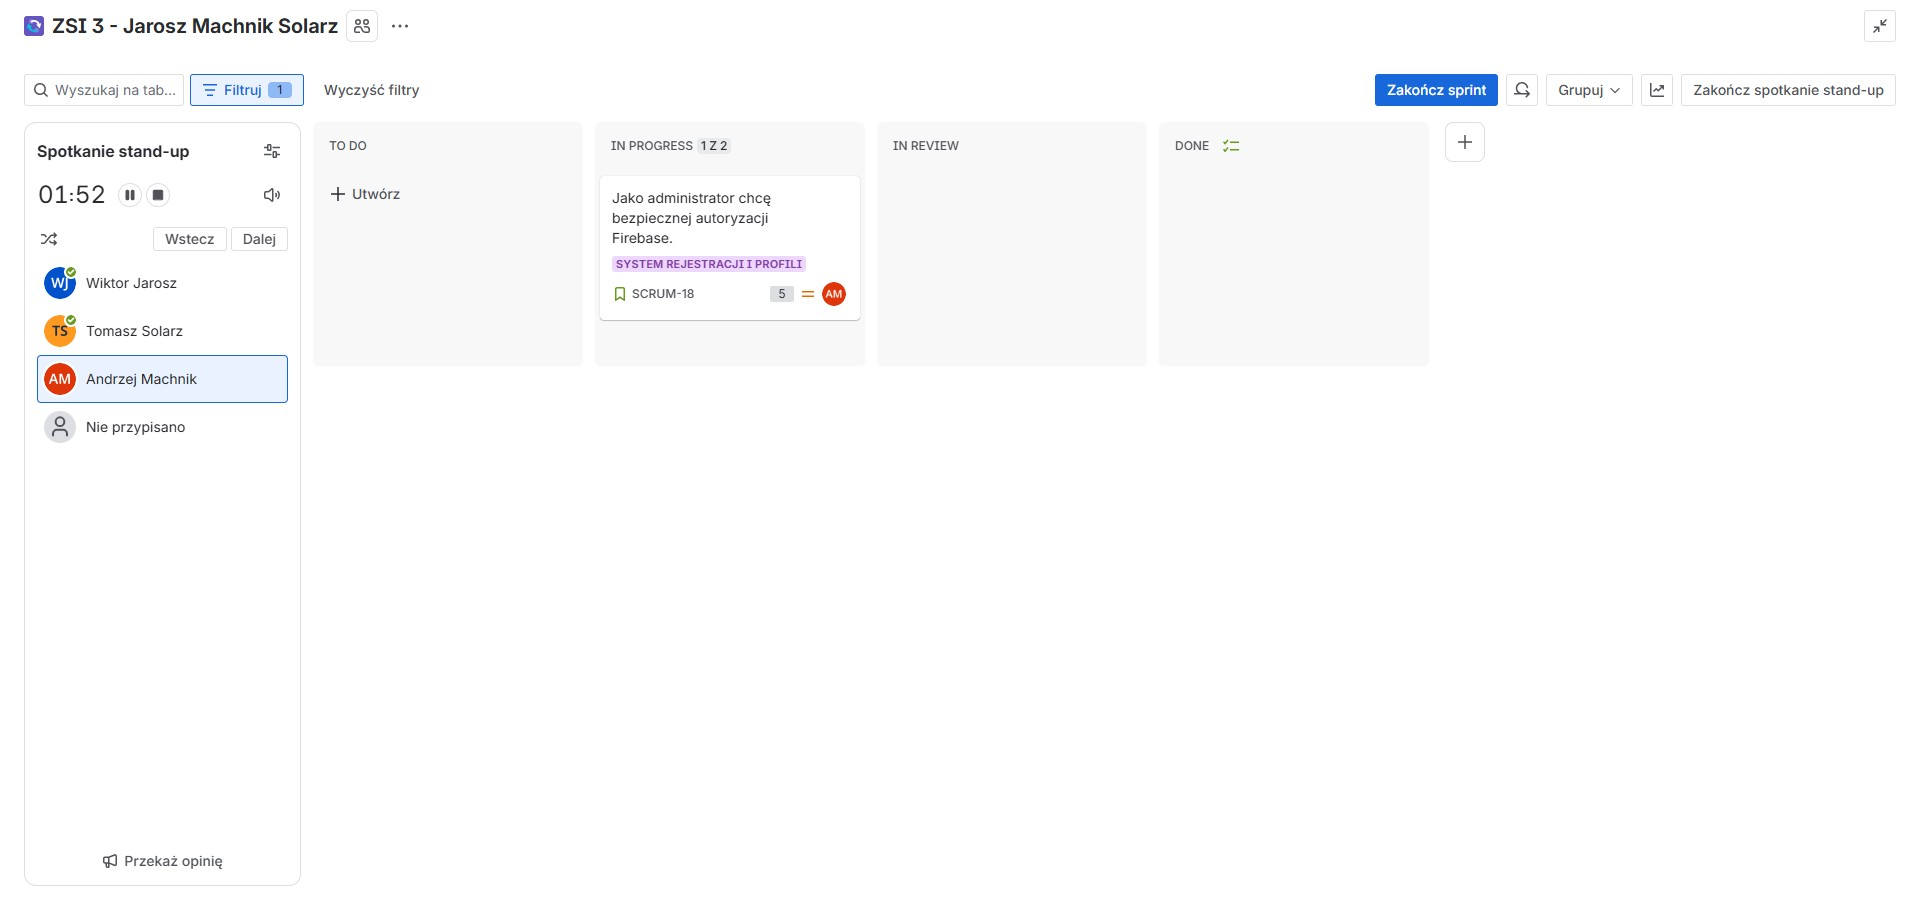
\includegraphics[width=0.8\linewidth]{../screeny/8.jpg}
		\caption{Podgląd tablicy filtrowanej pod kątem wybranego dewelopera podczas spotkania Stand-up}
		\label{fig:8}
	\end{figure}

	\begin{figure}[H]
		\centering
		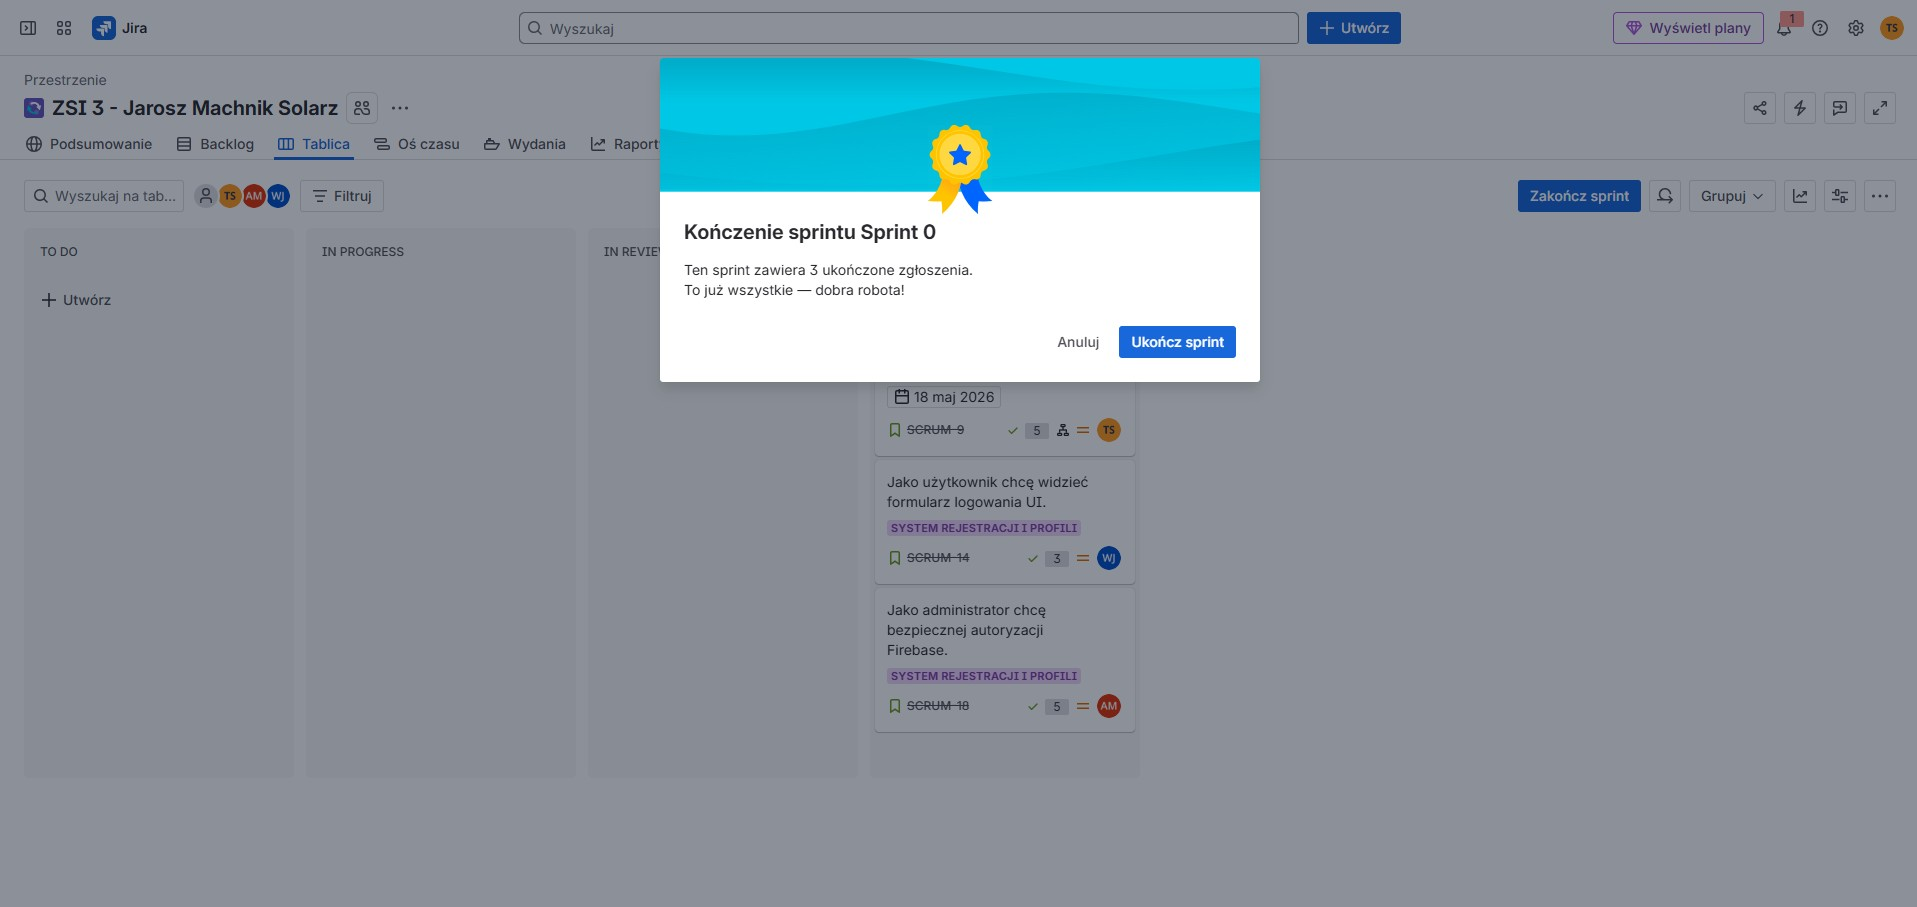
\includegraphics[width=0.8\linewidth]{../screeny/11.jpg}
		\caption{Podsumowanie i ukończenie wstępnego Sprintu 0}
		\label{fig:11}
	\end{figure}

	\begin{figure}[H]
		\centering
		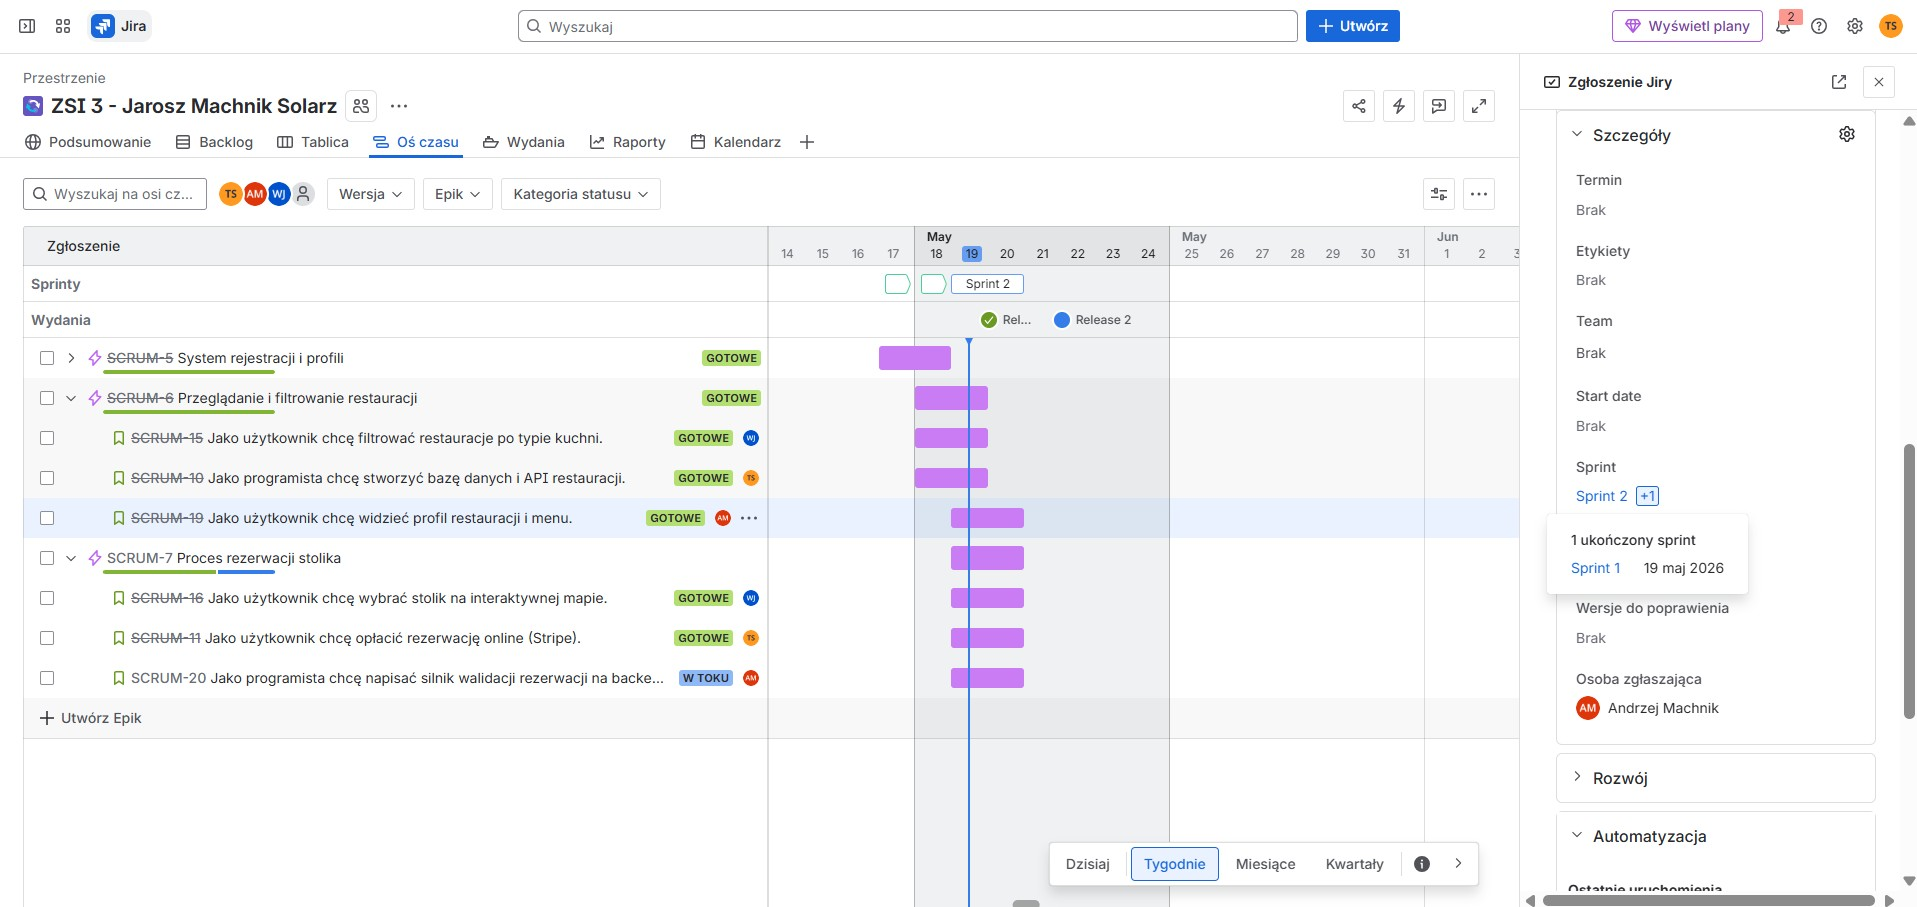
\includegraphics[width=0.8\linewidth]{../screeny/12.jpg}
		\caption{Oś czasu ukazująca zadanie nieukończone w terminie i przeniesione do kolejnego sprintu}
		\label{fig:12}
	\end{figure}

	\subsection{Raportowanie i analiza efektywności}
	Jira Software zapewniła rozbudowany wachlarz narzędzi do raportowania, co pozwalało realnie ocenić tempo pracy zespołu. Zakładka Kalendarza (Rysunek \ref{fig:13}) dostarczała syntetycznego widoku na harmonogram odbytych sprintów, wydanych releasów oraz wskazywała konkretne dni ukończenia historyjek.
	
	Wykres typu Burnup dla Sprintu 0 (Rysunek \ref{fig:14}) rzetelnie obrazuje zmiany w zakresie prac na przestrzeni czasu sprintu. Pionowy, czerwony skok linii na tym wykresie reprezentuje sytuację, kiedy niedoświadczony deweloper omyłkowo dobrał do sprintu więcej zadań niż wynosiło tzw. capacity zespołu (13 SP), co następnie wymagało ręcznej korekty i interwencji ze strony Scrum Mastera. Z kolei wykres spalania sprintu (Burndown) pochodzący ze Sprintu 2 (Rysunek \ref{fig:15}) ukazuje optymalne tempo wykonywania zadań w danym okresie czasu, na którym widoczne jest systematyczne ubywanie prac.
	
	Ostateczną weryfikacją skuteczności planowania zespołu był ogólny Raport o szybkości pracy (Velocity chart). Zobrazował on jasny stosunek wartości Story Points początkowo zadeklarowanych (szary słupek) do tych ostatecznie dostarczonych i uznanych za gotowe (zielony słupek). Na Rysunku \ref{fig:16} wyraźnie widać trudności estymacyjne w Sprincie 1, w którym zespołowi nie udało się dostarczyć wszystkiego, do czego się zobowiązał. Wykres ukazuje, że w Sprincie 0 pomyślnie dostarczono zadeklarowane 13 SP. Z kolei w Sprincie 1 nastąpił spadek efektywności wynikający ze zbyt optymistycznego zaplanowania prac. Wykres w naturalny sposób wyliczał uśrednione tempo dostarczania SP na przestrzeni odbytych iteracji. Całościowy, szeroki podgląd wszystkich realizowanych Epiców, wydań i odbytych prac na przestrzeni trzech sprintów ukazuje z perspektywy czasu główny widok Timeline (Rysunek \ref{fig:17}).

	\begin{figure}[H]
		\centering
		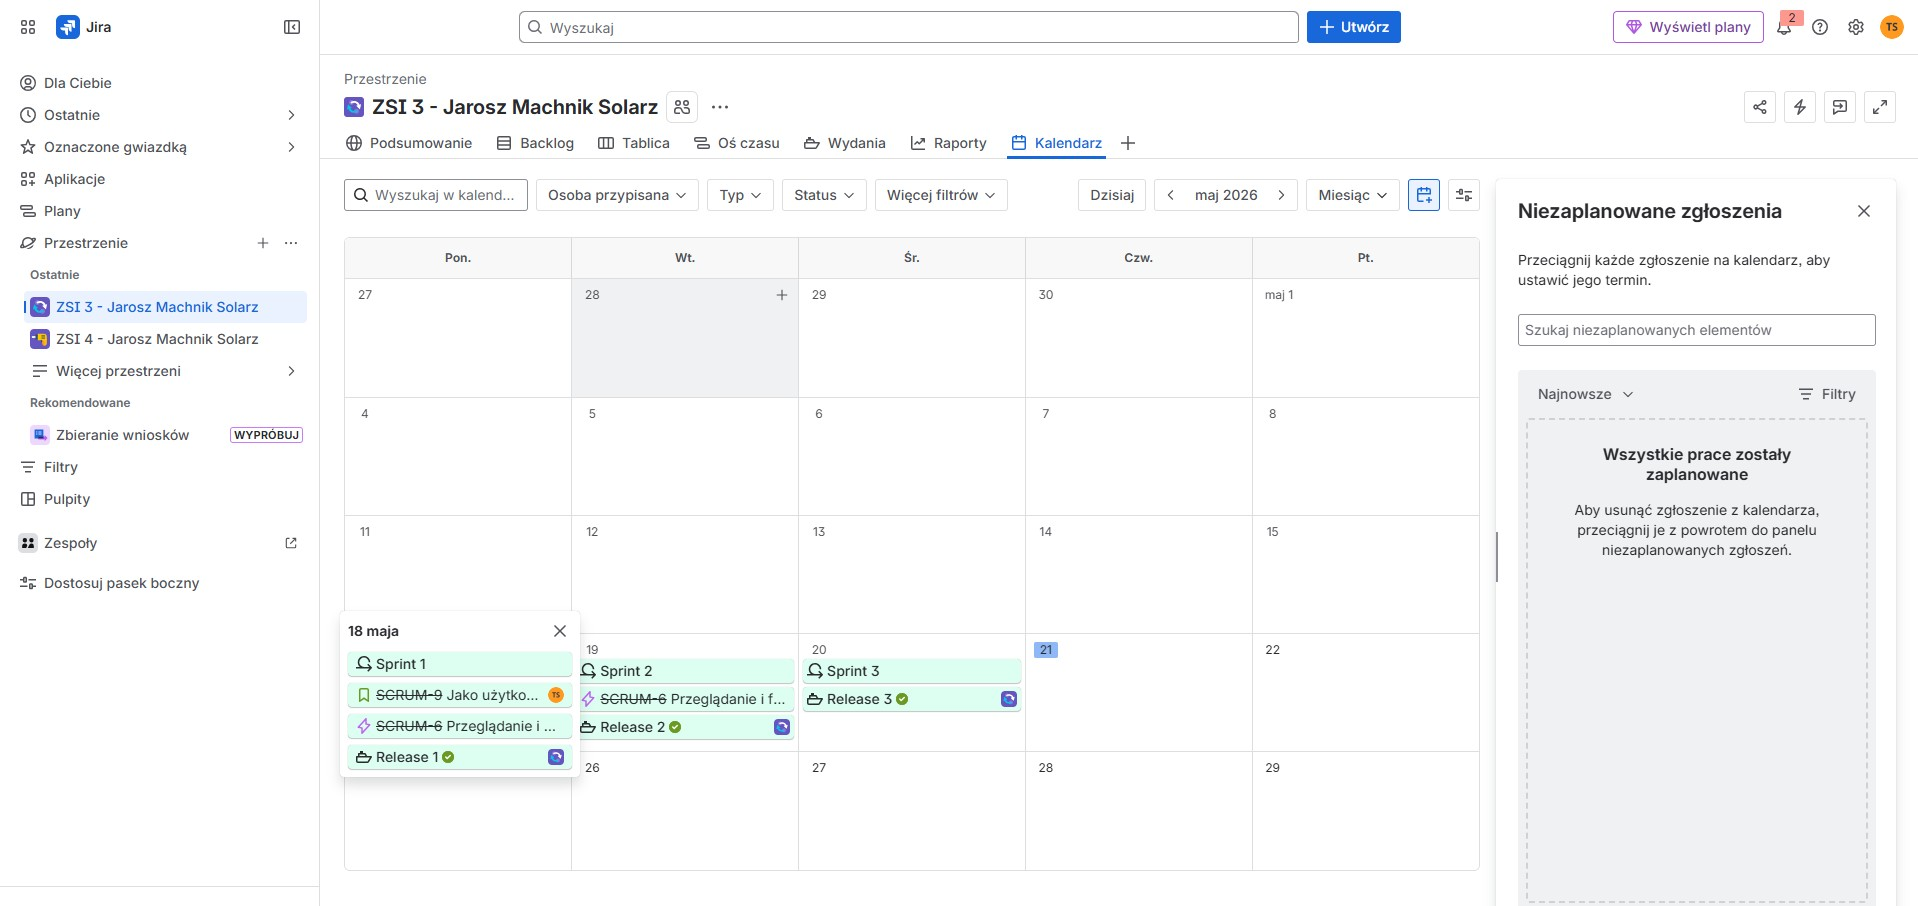
\includegraphics[width=0.8\linewidth]{../screeny/13.jpg}
		\caption{Widok zakłądki kalendarza prezentujący ukończone epici, historyjki oraz poszczególne sprinty}
		\label{fig:13}
	\end{figure}

	\begin{figure}[H]
		\centering
		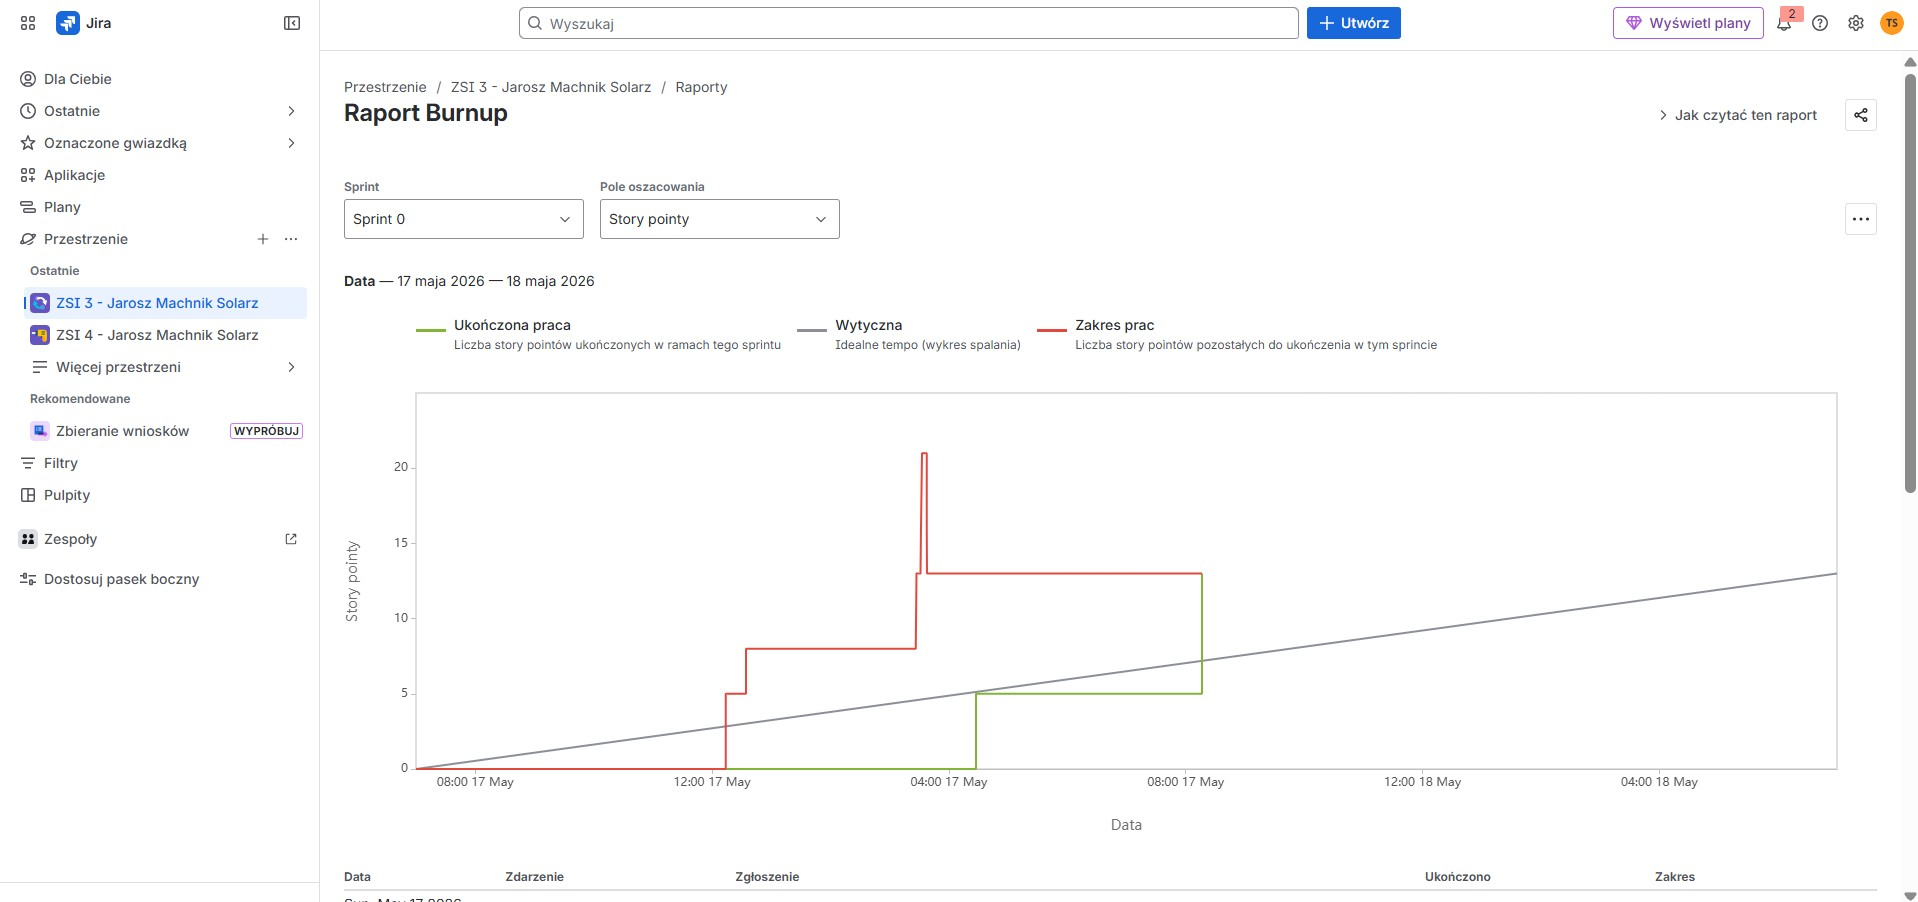
\includegraphics[width=0.8\linewidth]{../screeny/14.jpg}
		\caption{Raport Burnup ze Sprintu 0 ukazujący zakres prac i moment omyłkowego dołożenia zadań}
		\label{fig:14}
	\end{figure}

	\begin{figure}[H]
		\centering
		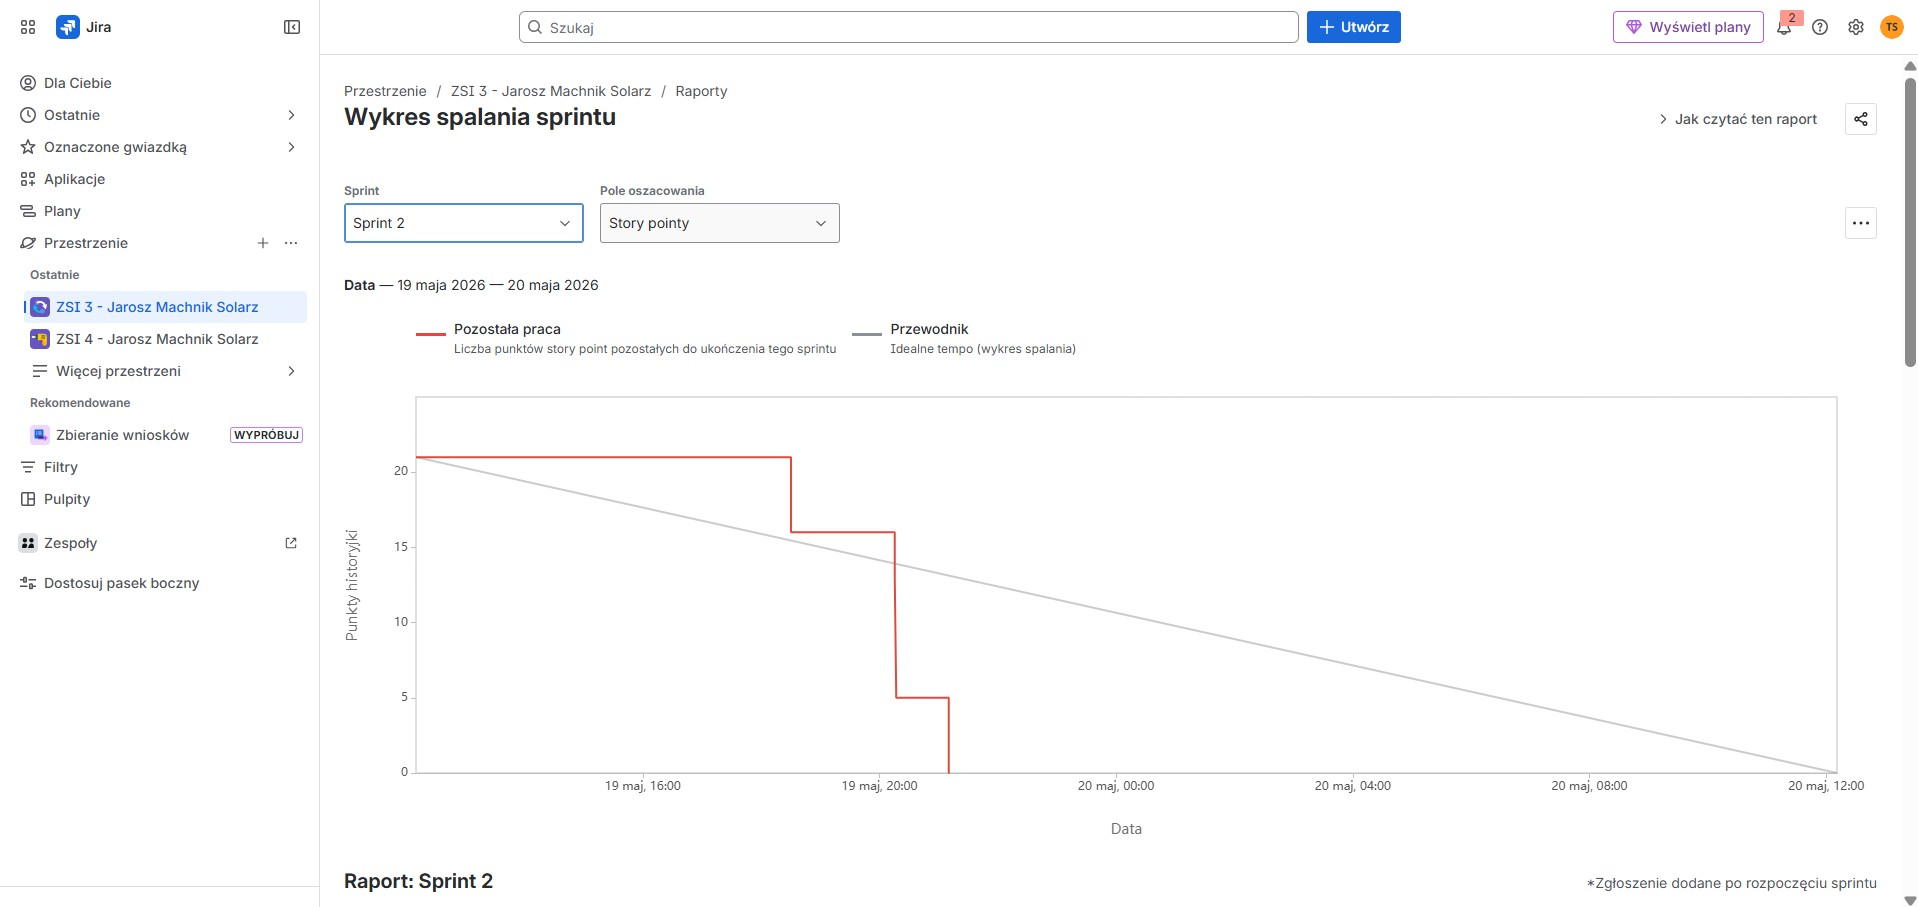
\includegraphics[width=0.8\linewidth]{../screeny/15.jpg}
		\caption{Raport z wykresem spalania sprintu (Burndown chart) w trakcie Sprintu 2}
		\label{fig:15}
	\end{figure}

	\begin{figure}[H]
		\centering
		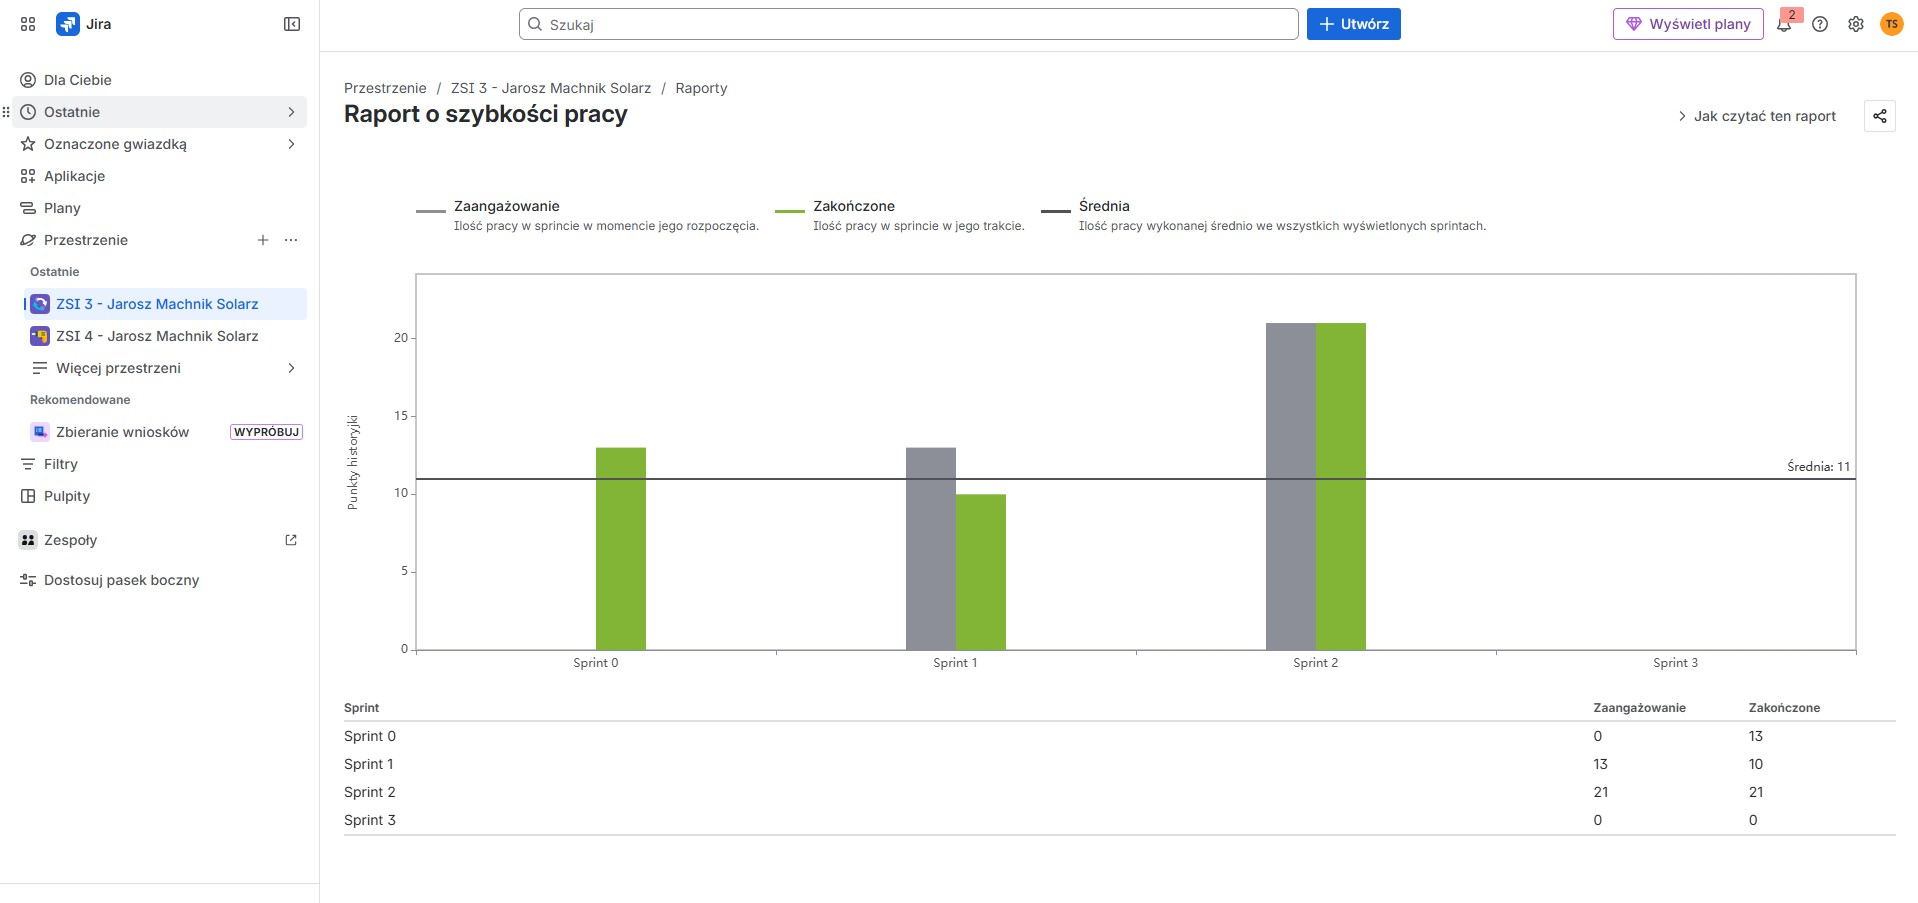
\includegraphics[width=0.8\linewidth]{../screeny/16.jpg}
		\caption{Raport szybkości pracy zespołu (Velocity chart) z wyliczoną średnią}
		\label{fig:16}
	\end{figure}

	\begin{figure}[H]
		\centering
		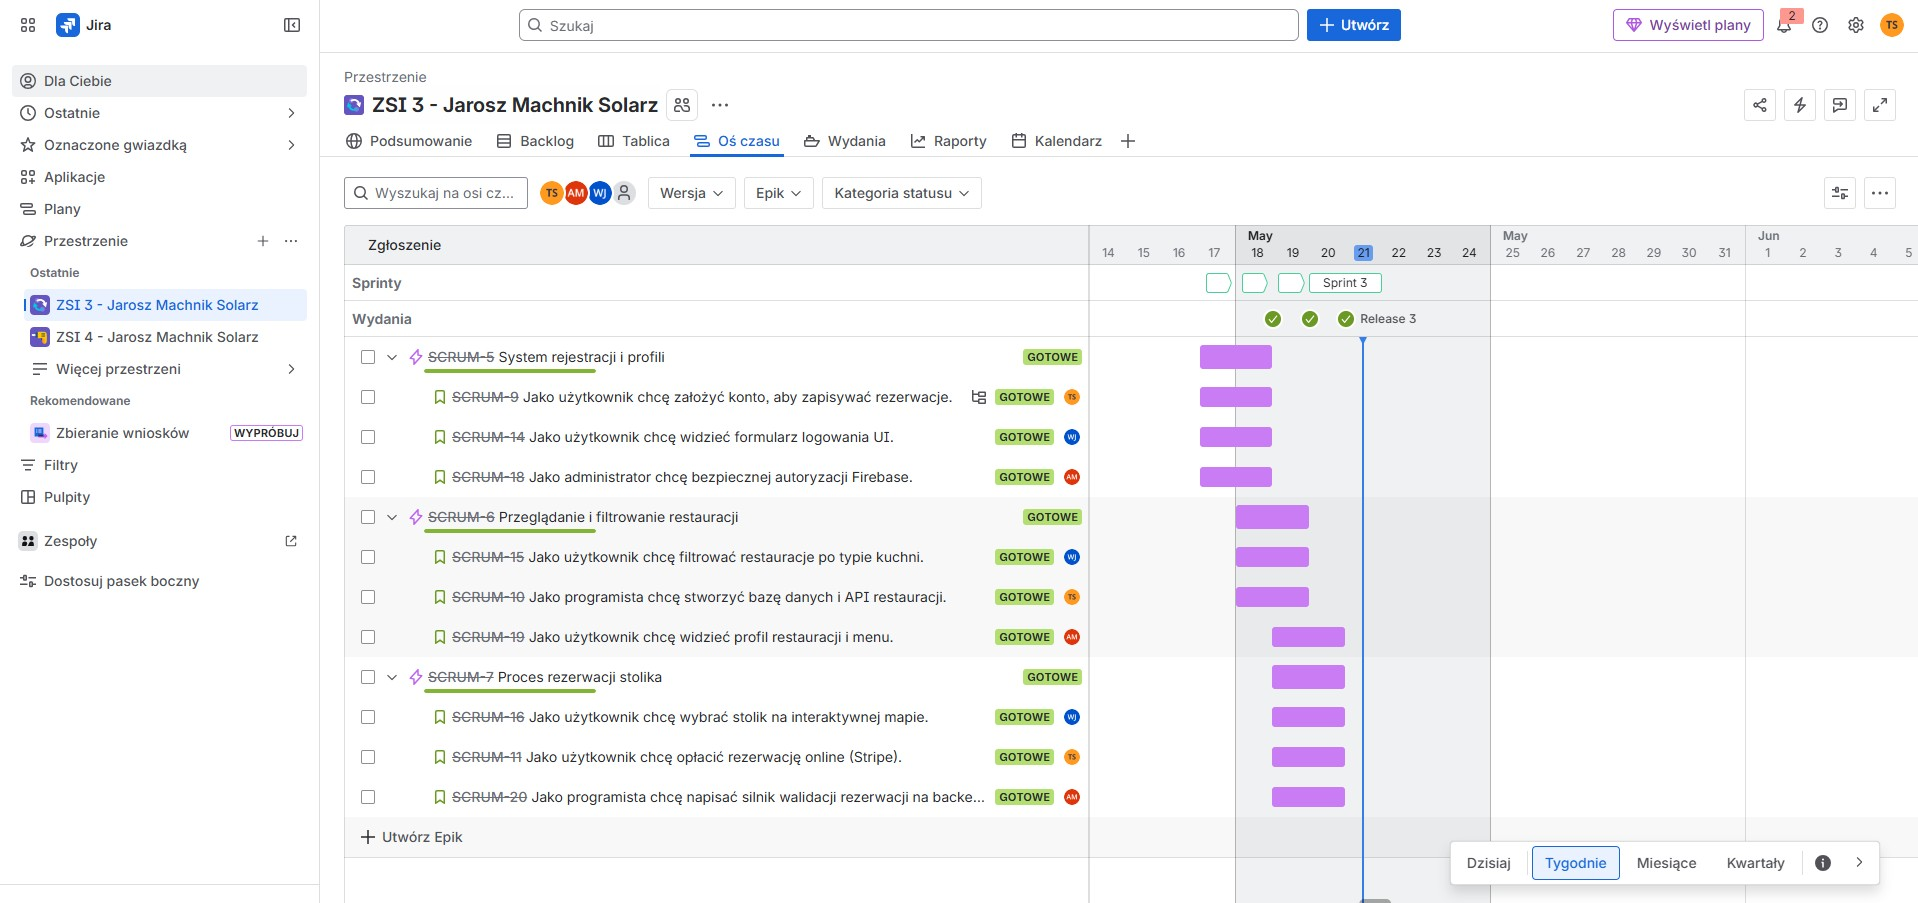
\includegraphics[width=0.8\linewidth]{../screeny/17.jpg}
		\caption{Oś czasu (Timeline) podsumowująca całościową pracę w trzech sprintach nad trzema wydaniami}
		\label{fig:17}
	\end{figure}





\newpage
\section{Wnioski}
	\begin{itemize}
		\item \textbf{Spostrzeżenia}: Aplikacja Jira to potężne narzędzie, które rewelacyjnie ułatwia śledzenie postępów prac oraz transparentną organizację. Zastosowanie w pełni wirtualnej tablicy redukuje koszty komunikacji, ale z drugiej strony wymaga dyscypliny i zrozumienia procesów przez cały zespół. Znaczące okazały się tu wnioski wyciągnięte chociażby po omyłkowym dodaniu zadań przez dewelopera w Sprincie 0, czy też przeszacowaniu możliwości zespołu w Sprincie 1.
		\item \textbf{Osiągnięcia}: Zespół z powodzeniem i zgodnie z planem wdrożył i przeprowadził symulowany cykl 3 iteracji (sprintów). Osiągnięto wymierną przewidywalność pracy, stabilizując Velocity zespołu po problemach początkowych (np. pomyślne dostarczenie 13 SP w Sprincie 0 oraz korekty planistyczne w kolejnych sprintach). Sukcesem było skonfigurowanie i wykorzystanie automatyzacji pozwalającej oszczędzać czas na powtarzalnych zadaniach weryfikacji. Oprócz tego na bieżąco analizowano postępy prac przy użyciu zaawansowanych raportów (Velocity, Sprint Burndown, Burnup), co na każdym kroku podnosiło świadomość członków zespołu w kwestii capacity.
		\item \textbf{Potencjał rozwoju}: Istnieje wiele dróg na ulepszenie stosowanych procesów. W kolejnych krokach rozbudowy struktury zarządzania warto byłoby zintegrować narzędzie Jira z używanym systemem kontroli wersji (takim jak GitHub lub GitLab). Istniałaby wtedy możliwość powiązania kodu źródłowego bezpośrednio z ticketami w backlogu. Skrypty automatyzacji można by także rozszerzyć o automatyczne asygnowanie konkretnych recenzentów po przeniesieniu zadania do kolumny \textit{In Review}.
	\end{itemize}





\newpage
\section{Bibliografia}
\begin{enumerate}
	\item \textit{Dokumentacja użytkownika i baza wiedzy Atlassian Jira} (\url{https://confluence.atlassian.com/jira})
	\item \textit{The Scrum Guide (\url{https://scrumguides.org/docs/scrumguide/v2020/2020-Scrum-Guide-US.pdf})}, Schwaber K., Sutherland J.
\end{enumerate}

\end{document}
